%!TEX root = ../thesis.tex
%*******************************************************************************
%****************************** Second Chapter *********************************
%*******************************************************************************

\chapter{Single molecule somatic mutation detection}

\ifpdf
    \graphicspath{{Chapter2/Figs/Raster/}{Chapter2/Figs/PDF/}{Chapter2/Figs/}}
\else
    \graphicspath{{Chapter2/Figs/Vector/}{Chapter2/Figs/}}
\fi

\section{Introduction}

\textit{Most sequences have been derived by priming on both strands; this allows more confidence than when only one strand could be used} 
\begin{flushright} (Frederick Sanger, 1977 \cite{Sanger1977-os}) \end{flushright}


As described in chapter 1, both duplex and CCS sequencing leverages redundant sequencing and complementary base pairing between the forward and reverse strand of a double-stranded DNA molecule to create a highly accurate consensus sequence. Considering the similarities between duplex and CCS sequencing \cite{Schmitt2012-yr, Hoang2016-jx, Abascal2021-pk}, I hypothesised that CCS reads might be as accurate or more accurate than duplex reads and that they can be used for single molecule somatic mutation detection. If my hypothesis proves to be true, somatic mutation detection and mutational signature identification will be possible from CCS sequencing of a bulk normal tissue. 

\subsection{Sanger sequencing}

The duplex sequencing method was introduced right at the start of DNA sequencing by Frederick Sanger and colleagues and was used to determine 5,735bp $\Phi$X174 genome sequence \cite{Sanger1977-os}. The bi-directional Sanger sequencing method primes and sequences both strands of a double-stranded DNA molecule to generate bases with higher base accuracy. 

\subsection{Duplex sequencing}

The current incarnation of the duplex sequencing method takes advantage of the higher sequence throughput of the Illumina platform to increase the base accuracy of short reads and to enable ultra-rare somatic mutation detection (<0.01\% variant allele fraction (VAF)) \cite{Schmitt2012-yr}. The higher base accuracy is required to distinguish recently acquired somatic mutations from stochastic sequencing errors. Hence, the base accuracy determines the VAF threshold at which somatic mutations can be accurately detected. 


The duplex library preparation protocol starts with the sonication and fragmentation of genomic DNA. Unique molecular identifier (UMI) consisting of 8 to 12 nucleotides and Illumina adapters are attached to double-stranded DNA molecules prior to their PCR amplification \cite{Schmitt2012-yr}. The duplex library is diluted before PCR amplification to achieve optimal sampling and duplication per template molecule \cite{Hoang2016-jx, Abascal2021-pk}. Illumina reads from the library are subsequently grouped according to their UMI and are classified as Watson or Crick strand depending on whether the sequence was derived from the P5 or P7 Illumina adapter, respectively. 

A highly accurate duplex consensus sequence is, thereafter, generated taking advantage of the redundancies and complementary base pairing between the forward and reverse strand reads (Figure \ref{figure:duplex-sequencing}). 

\begin{figure}[htbp!]
\caption{Duplex sequencing}
\label{figure:duplex-sequencing}
\begin{centering}
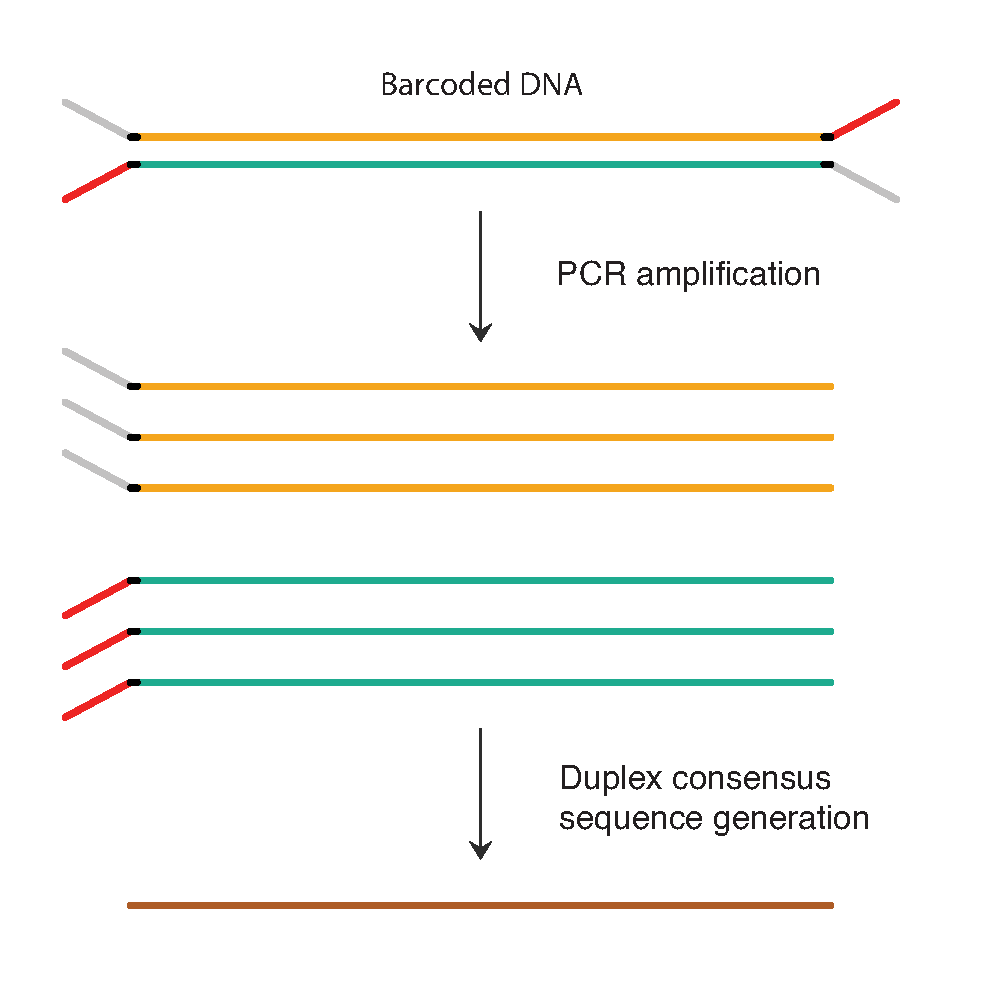
\includegraphics[width=0.55\textwidth]{Vector/duplex_sequencing.pdf}
\end{centering}
\floatfoot{A double-stranded DNA with a UMI and Illumina library adapters are PCR amplified. The forward strand is in yellow and reverse strand is in green. Strand orientation of the read is determined from the Illumina adapter.}
\end{figure}

The higher sequence throughput of Illumina instruments is critical in acquiring multiple reads from both strands of the template molecule and to identifying library and amplification errors introduced upstream of sequencing. DNAP, for example, might incorrectly replicate the template DNA molecule during PCR amplification, but the polymerase error will be present only in one copy or a subset of the copies. Moreover, if both forward and reverse strands are adequately sampled, complementarity between the two strands can be leveraged to identify bases with high accuracy or \cite{Schmitt2012-yr} or estimate the base accuracy \cite{Abascal2021-pk} based on supporting bases and the associated base quality scores. Duplex reads, therefore, promises theoretical base accuracy of $1 \times 10^{-9}$ (Q90), although in practice duplex reads achieves a base accuracy of $1 \times 10^{-6}$ (Q60) \cite{Schmitt2012-yr}.

\subsection{Nanorate sequencing}

In contrast, duplex reads from the most recent nanorate library protocol achieve the promised Q90 base accuracy, which is sufficient for single-molecule resolution somatic mutation detection \cite{Abascal2021-pk} (the name of the protocol is derived from the error rate of 1 error per billion bases). To accomplish this, the nanorate library protocol reduces library errors upstream of PCR amplification, and duplex libraries are created from DNA molecules assumed to be free of errors. Blunt end restriction enzyme, for example, is used to fragment gDNA to prevent enzymatic DNA misincorporation during end-repair and gap-filling. In addition, dideoxynucleotides are added to terminate single-strand displacement synthesis through nick translation, rendering DNA molecules that require this process unsuitable for library creation. A highly accurate duplex read, thereafter, is constructed as described above.  

\subsection{CCS sequencing}

CCS sequencing like duplex sequencing generates a highly accurate consensus sequence from multiple pass sequencing of a double-stranded DNA molecule. The single-strand reads are referred to as subreads and an individual subread typically has 10-15\% error rate \cite{Chaisson2012-vr}. CCS reads are reported to have an average read accuracy above Q20 \cite{Wenger2019-pw}, but their individual base accuracies have not been examined to date. I and others have previously hypothesised that PacBio circular consensus sequence (CCS) reads could have sufficient base accuracy for single-molecule resolution somatic mutation detection \cite{Salk2018-cp}. CCS library preparation also benefits from the absence of PCR jackpot errors that occur at the earliest stage of PCR amplification. Given that the commercial CCS library preparation protocol has greater similarity to the duplex sequencing protocol \cite{Schmitt2012-yr} than the nanorate library protocol \cite{Abascal2021-pk}, CCS reads are hypothesised to have a base accuracy between that of duplex reads generated from the former and the latter methods. CCS library preparation protocol like the duplex sequencing protocol uses several DNA damage repair enzymes and erroneous repair of DNA damage can be a source of false positive somatic mutation calls. 

The PacBio circular consensus sequence (pbccs) algorithm assigns to each called base BQ score that ranges from Q1 to nominal Q93, representing an error rate of 1 error per billion bases. If the BQ score were correct, single molecule-resolution somatic mutation detection would be possible across most human normal tissue. Among the human tissue, colonic crypt has one of the highest somatic mutation rate (around 40 substitutions per cell per year) \cite{Lee-Six2019-vt} and spermatogonium has the lowest somatic mutation rate (approximately 2.9 substitutions per cell per year) \cite{Rahbari2016-ot}. In addition, haematopoietic stem cells (HPSC), one of the most accessible samples, accumulates roughly 16.8 somatic substitutions per cell per year. \cite{Osorio2018-mh, Mitchell2022-ry}. A normal human genome without defects in DNA damage repair pathway, therefore, acquires somatic substitution at a rate between Q82 and Q93 per year and gains hundreds to thousands of somatic mutations across a lifetime. Hence, in a normal sample, the somatic mutations should outnumber of the number of false positives from Q93 CCS bases and ongoing somatic mutational process should be directly observable from the mutational spectrum.  

In contrast to duplex sequencing, CCS sequencing also offers several advantages for somatic mutation detection. Firstly, bulk normal CCS sequencing enables simultaneous genome-wide detection of both germline and somatic mutations. On the other hand, duplex sequencing requires a matched normal sequencing to distinguish germline mutations from somatic mutations and somatic mutation detection is limited to where a blunt-ended restriction enzyme recognition site is available \cite{Abascal2021-pk}. Secondly, the longer read length ($\sim$10-20kb) combined with higher base accuracy enable accurate read placement and differentiation of more recently diverged repeats, such as segmental duplications, from one another. Finally, given that the read length of a CCS read is long enough to span at least one heterozygous SNP (hetSNP), most somatic mutations could also be haplotype phased. 

\subsection{Sources of CCS errors}

Single-molecule resolution somatic mutation detection requires only a single read, derived from a single molecule of double-stranded DNA, to support the mismatch between the sample and the reference genome. CCS library preparation, sequencing and consensus sequence generation, processes upstream of downstream sequence analysis, can generate errors and these errors can be often misclassified as somatic mutations \cite{Cibulskis2013-gw}. Compared to paired tumour-normal sequencing, single molecule somatic mutation detection from normal tissues has a greater risk of mislabelling errors as somatic mutations. Furthermore, in samples with high heterozygosity and low sequence coverage, there is a possibility of miscategorising heterozygous mutations as somatic mutations. Here, I detail the potential sources of errors and I address some of these errors in the results section.

\subsubsection{Library and sequencing errors}

CCS library preparation begins with HMW DNA extraction using either Qiagen Magattract or Circulomics HMW DNA extraction kit. If an adequate amount of HMW DNA has been extracted, HMW DNA is sheared to the appropriate size using a Megaruptor instrument. Subsequently, end-repair and poly(A) tailing is performed to remove protruding ends and facilitate adapter ligation, respectively. A hairpin adapter is attached to both ends of the double-stranded DNA molecule to create a topologically circular template, called a SMRTbell template. BluePippin based size selection may additionally be performed to prepare size-selected libraries to maximise sequence throughput per SMRTcell. 

During CCS library preparation, A DNA damage repair enzyme cocktail (unpublished) is to repair DNA damage (nicks, abasic sites, thymidine dimers, blocked 3’-ends, oxidised guanine, and pyrimidines and deaminated cytosines) introduced before and during library preparation (personal communication with Jonas Korlach, Chief Scientific Officer at PacBio). In addition, DNA nuclease is subsequently used to digest DNA molecules not suitable for sequencing (e.g, failed ligation products). Defective DNA damage repair or unrepaired DNA damage can be misclassified as a somatic mutation. As discussed above, nanorate sequencing protocol pinpoints end-repair and nick-translation as the principal causes of duplex library errors \cite{Abascal2021-pk}. Considering the similarities between duplex and CCS sequencing protocol, similar processes are assumed to be the primary sources of library errors.

After CCS library preparation, SMRTbell templates are loaded onto the SMRTcell, whereupon template DNA molecules diffuses into one of the available ZMWs. PacBio defines a ZMW as a productive if and only if it has a single template molecule and if it generates a CCS read with at least Q20 read accuracy. DNAP at the bottom of the ZMW binds to the DNA primer and initiates rolling circle amplification through strand-displacement synthesis. DNAP incorporates fluorescently labelled nucleotides, fluorescence emitted during DNA incorporation is measured and fluorophore is cleaved off upon successful incorporation. The wavelength of the fluorescence, length of the fluorescence, and duration between the successive pulses of fluorescence are used to determine the identity of the base and chemical modifications to the base. If the detected fluorescence pulse is too short or too long compared to the expected fluorescence pulse from the template molecule, erroneous deletions or insertions can be introduced to the polymerase reads \cite{Eid2009-ol} and 1bp indel errors are common in homopolymer regions \cite{Chaisson2012-vr}. 

The DNAP from the latest library protocol has sufficient processivity to generate an average of 10-12 full-length subreads on average for template molecules with read-of-insert length between 16kb and 20kb. The single-strand readouts of the forward and reverse strand of the template molecule are referred to as subreads and individual subreads are reported to have 10 to 15\% error rate \cite{Chaisson2012-vr}. The first subread and the last subread are often partial readouts of the template molecule resulting from internal priming and early sequencing termination respectively, while the subreads from the second to the penultimate subreads are full-length readouts of the template molecule.

\subsubsection{Software errors}

To construct CCS reads, PacBio circular consensus sequence (pbccs) algorithm identifies and removes adapter sequences from polymerase reads, and uses the adapter sequences to demarcate the start and end of subreads (Figure \ref{figure:adpater-sequence-detection}). 

\begin{figure}[htbp!]
\caption{Adapter sequence detection}
\label{figure:adapter-sequence-detection}
\begin{centering}
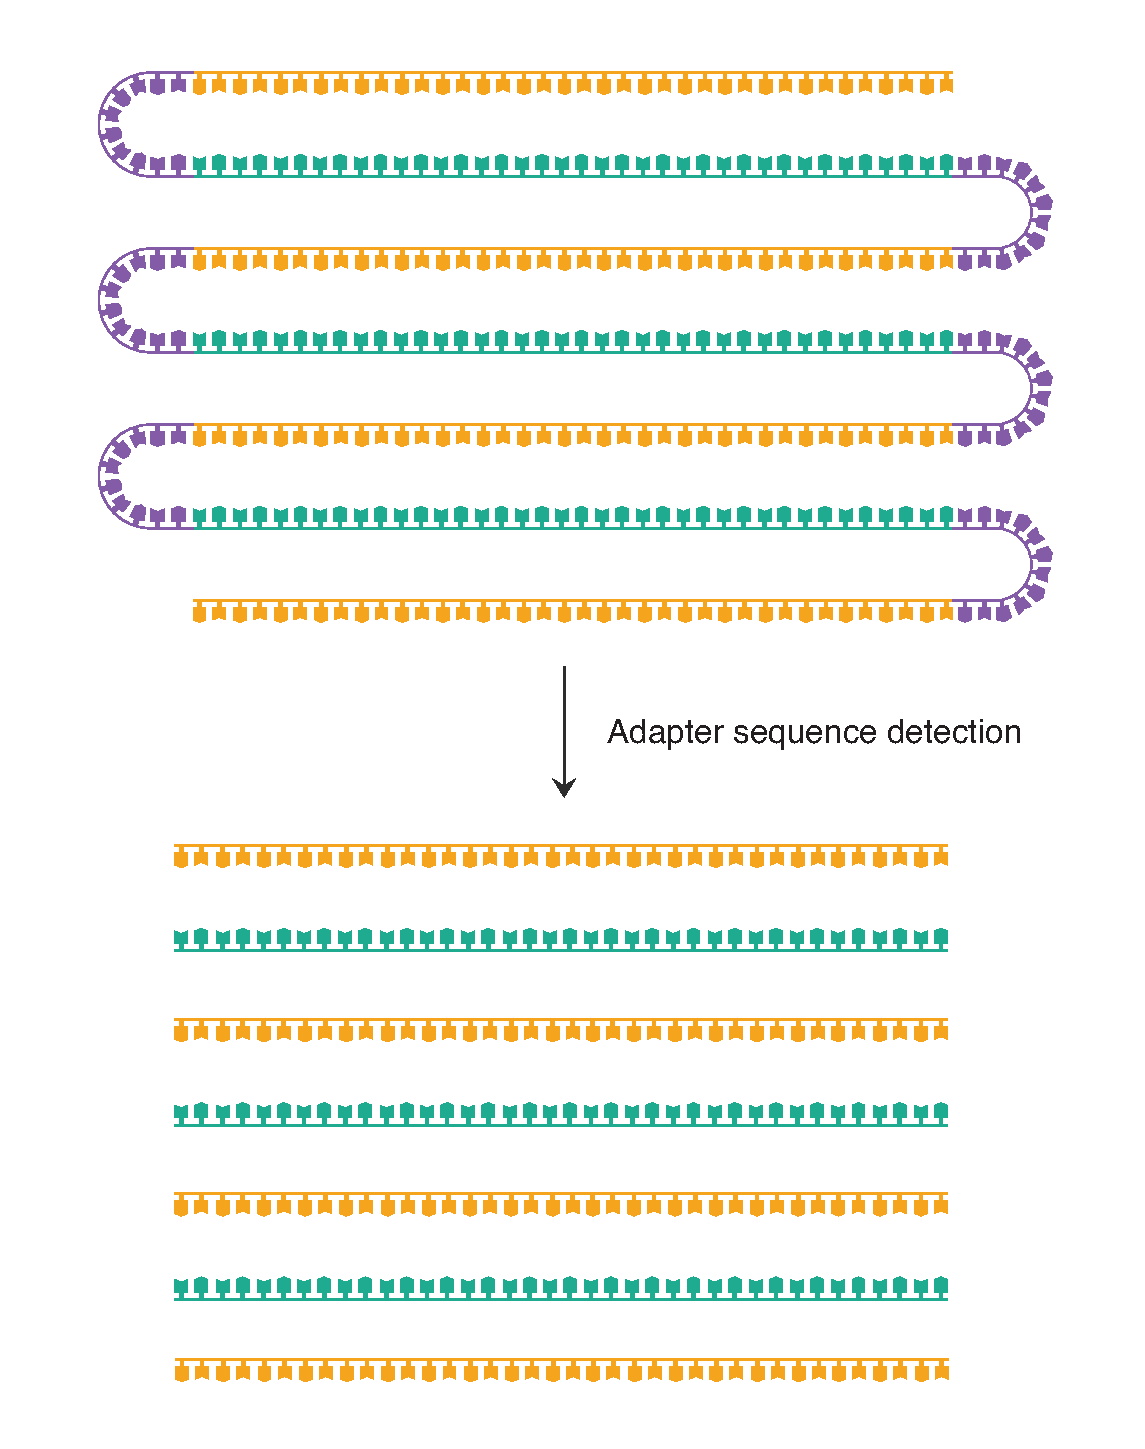
\includegraphics[width=0.5\textwidth]{Vector/adapter-sequence-detection.pdf}
\end{centering}
\floatfoot{A hairpin adapter in purple detected from the polymerase read to create subreads.}
\end{figure}

Afterwards, the median subread length is calculated and subreads with read length between 50\% of median subread length and 200\% of median subread length are used for consensus sequence generation. A sparse k-mer graph is generated from the subreads and a draft consensus sequence is inferred from the path with the highest confidence \cite{Ye2016-qe}. To polish the draft consensus sequence, subreads are realigned to the draft consensus sequence and A dinucleotide sequence context Hidden Markov Model (HMM) is used to infer the correct base and to assign base quality (BQ) scores from the observed subread bases (personal communication with Aaron Wenger, principal scientist at PacBio). A highly accurate consensus sequence can be constructed as sequencing errors are thought to be randomly introduced without sequence context bias and are independent of each other (Figure \ref{figure:ccs-generation}). In addition, non-complementary base pairing between the forward and reverse strand indicates the presence of an error and CCS base resulting from the heteroduplex is assigned a low BQ score \cite{ccs2023}. 

\begin{figure}[htbp!]
\caption{CCS generation}
\label{figure:ccs-generation}
\begin{centering}
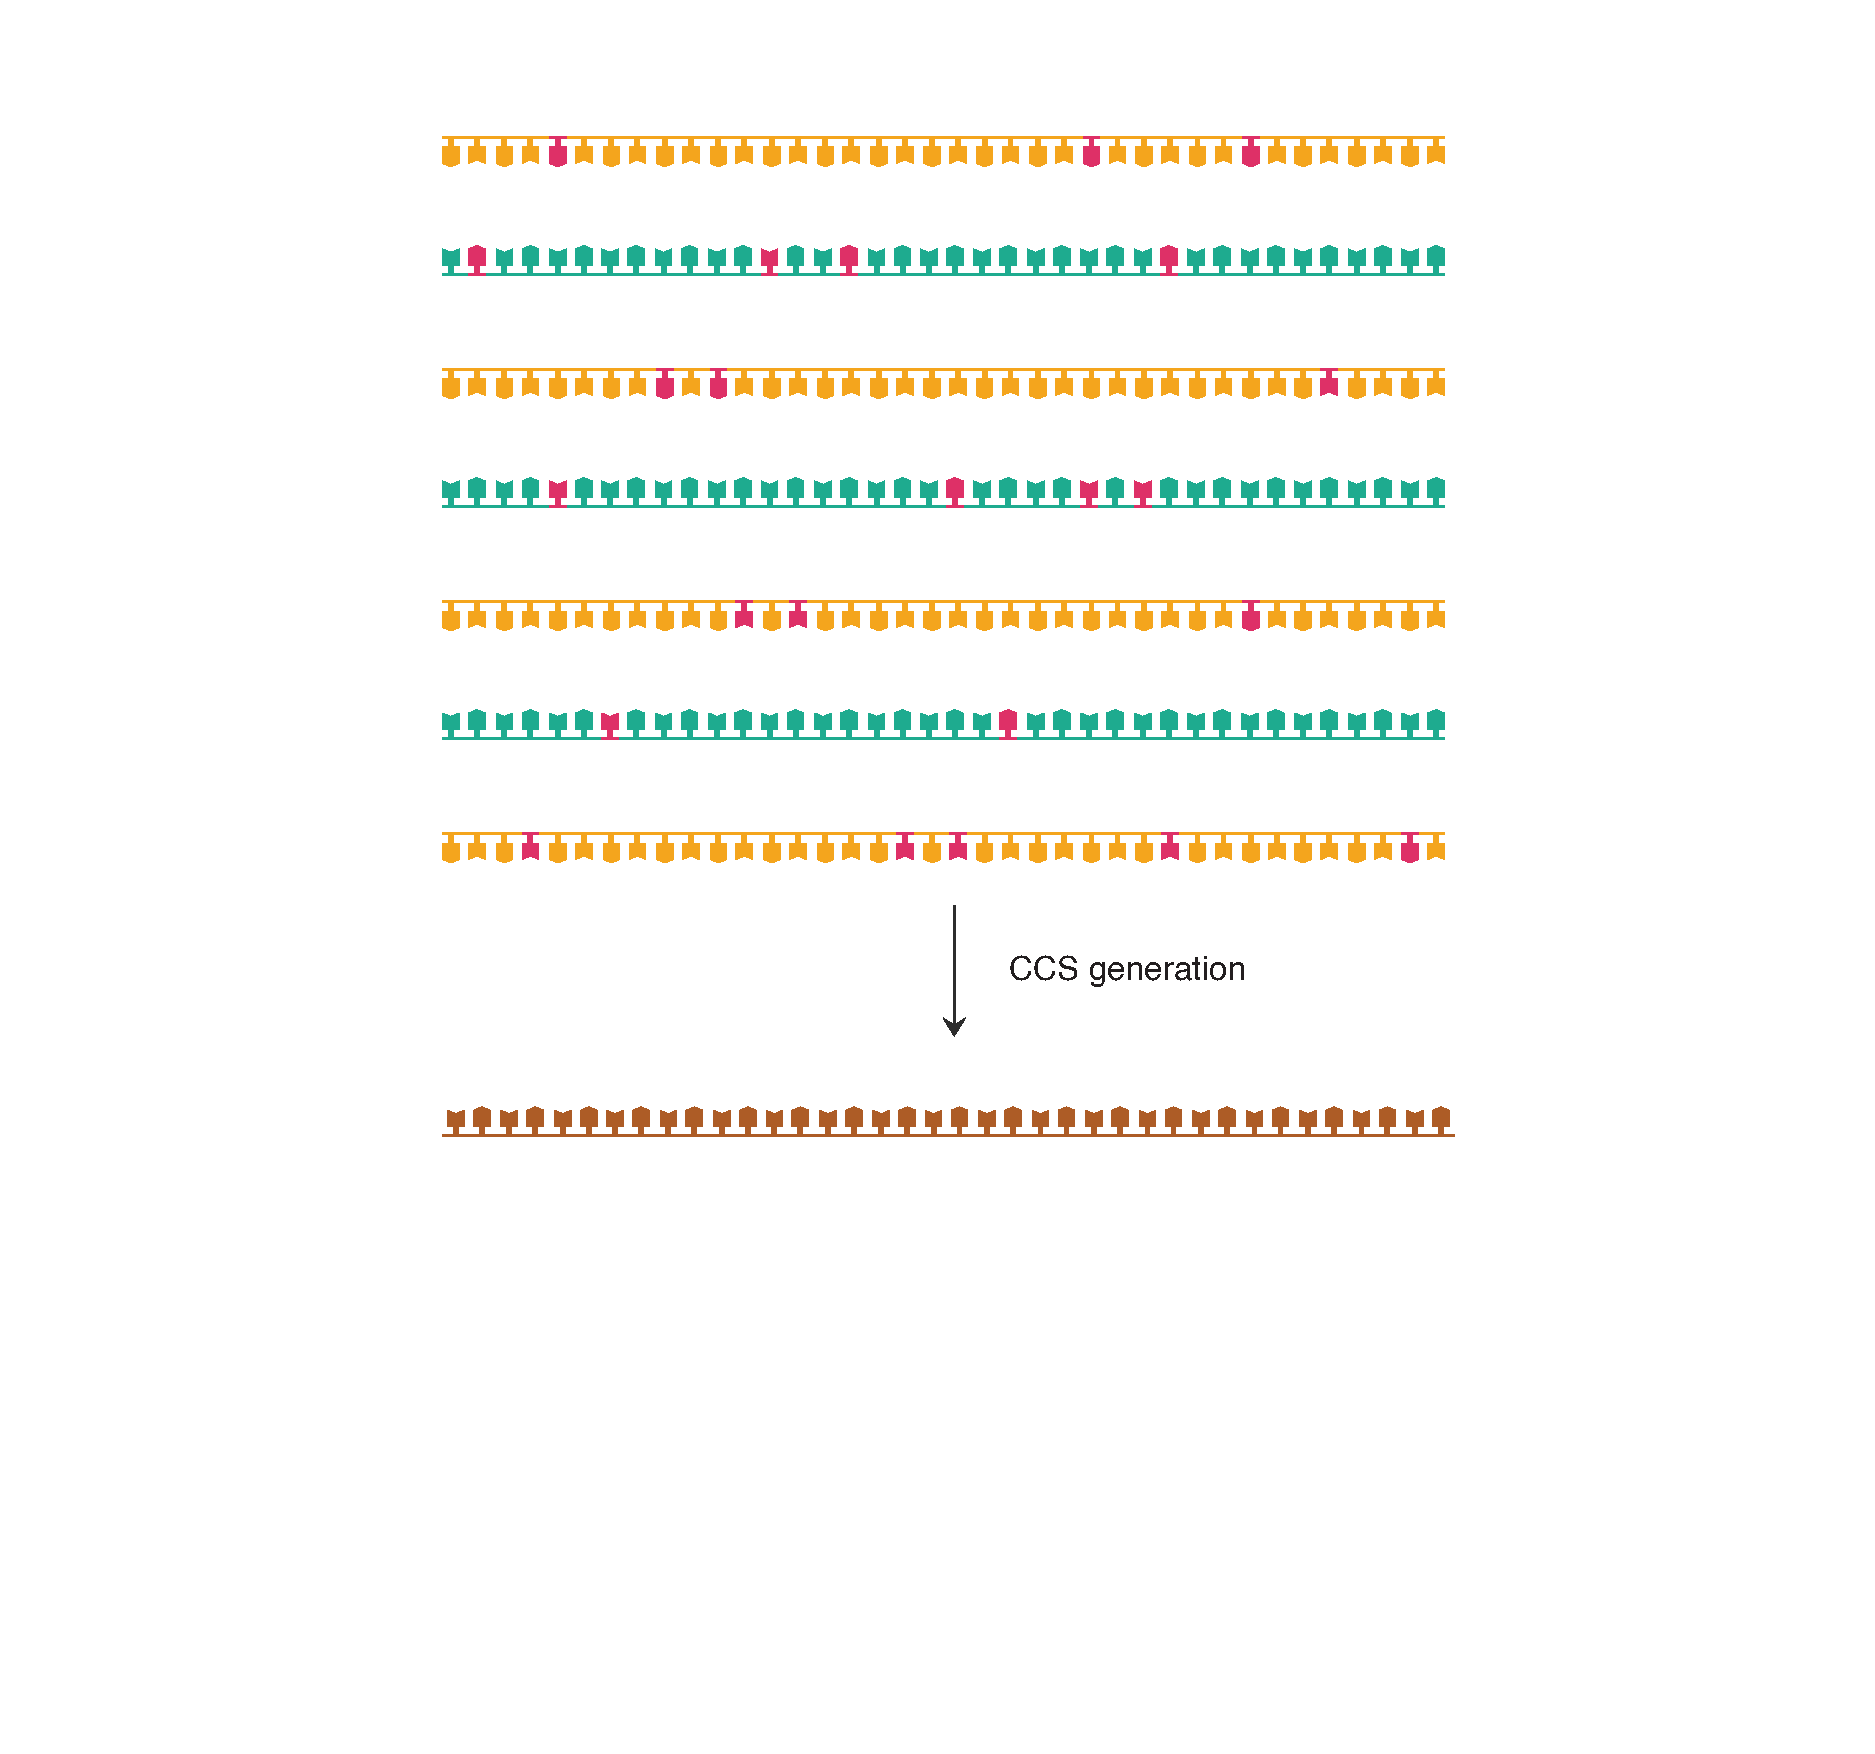
\includegraphics[width=0.5\textwidth]{Vector/ccs-generation.pdf}
\end{centering}
\floatfoot{Subreads, in green and yellow, derived from a double-stranded DNA molecule is used to generate a highly accurate consensus sequence, in brown, with at least Q20 read accuracy. The bases colour coded in red are sequencing errors introduced randomly to the subreads. }
\end{figure}

Data processing and software design errors also have the potential to introduce false positive mutations during downstream sequence analysis. If adapter sequences are not trimmed properly from subreads, adapter sequences can be incorporated into CCS reads and alignment errors arising from the adapter sequence can be a source of false positive mutations. 

\begin{figure}[htbp!]
\caption{Subread fragmentation}
\label{figure:subread-fragmentation}
\begin{centering}
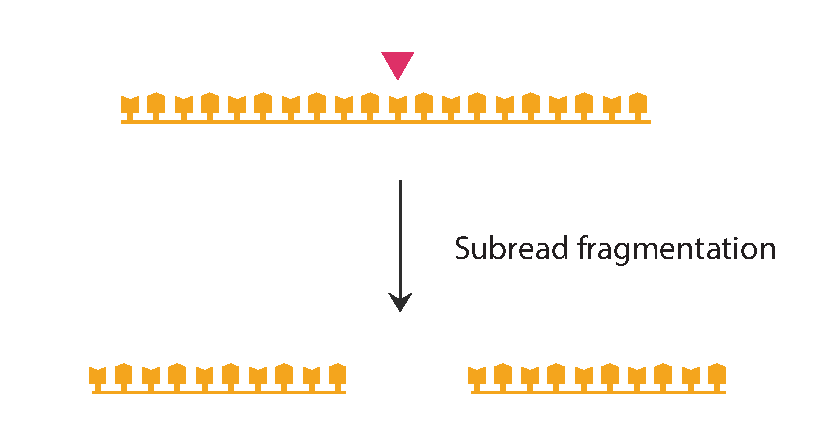
\includegraphics[width=0.5\textwidth]{Vector/subread-fragmentation.pdf}
\end{centering}
\floatfoot{The red triangle indicates where adapter sequence has been miscalled in the subread, resulting in two partial subreads}
\end{figure}

Furthermore, pbccs algorithm currently uses a hard filter to distinguish full-length subreads from subreads where adapter sequence has been miscalled, but a hard filter is not an adequate classification method.  If adapter sequences are inappropriately detected within a subread or not detected where present, full-length subreads can be fragmented into multiple subreads (Figure \ref{figure:subread-fragmentation}) and more than two subreads can be concatenated into a single subread, respectively (Figure \ref{figure:subread-concatenation}).

In some cases, fragmented and concatenated subreads are also joined together to produce a subread with sequences from both the forward and reverse strand. Moreover, as DNAP is agnostic to strand orientation, odd-numbered and even-numbered subreads are often assumed to have the same sequence orientation. If adapter sequences are miscalled, this assumption does not hold true, and documentation does not detail how these edge cases are considered.

\begin{figure}[htbp!]
\caption{Subread concatenation }
\label{figure:subread-concatenation}
\begin{centering}
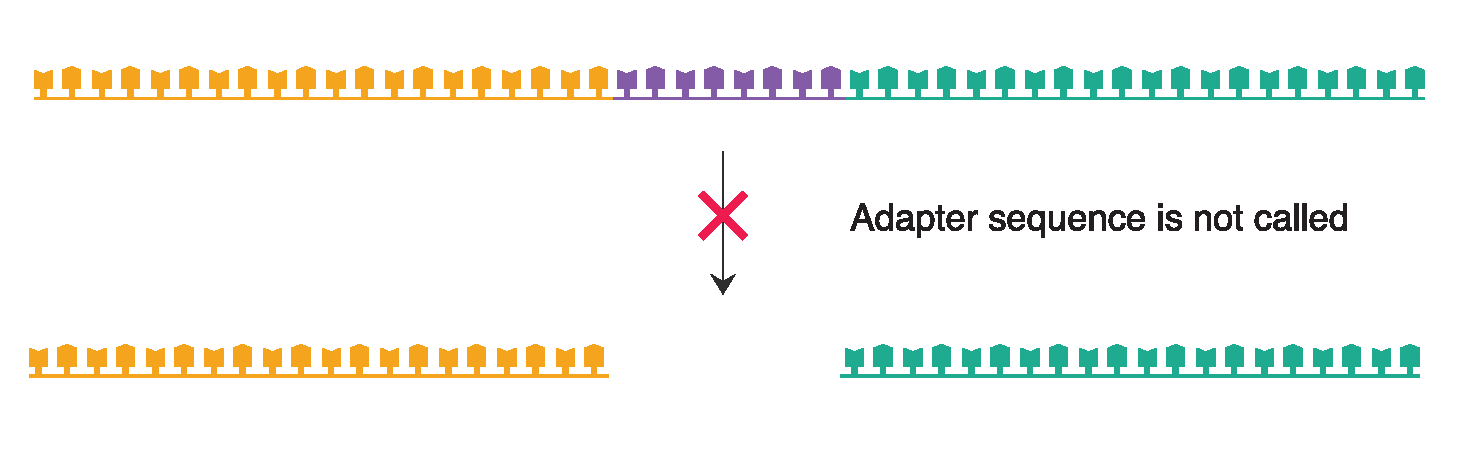
\includegraphics[width=0.7\textwidth]{Vector/subread_concatenation.pdf}
\end{centering}
\floatfoot{If adapter is not called where present, two subreads with different sequence orientation can be connected to a single subread.}
\end{figure}

\subsubsection{Samples with a single somatic mutational process}

Single molecule somatic mutation candidates are generated from either a biological process or from library, sequencing, or bioinformatics errors. To determine whether single molecule somatic mutation detection is possible with CCS reads, I selected a set of samples with a single somatic mutational process with characterised mutational signatures as positive controls and a sample with few somatic mutations as a negative control. In contrast to a typical sample where multiple mutational processes might be active at any given time, single-cell clone expansion and sequencing studies have identified APOBEC, POLE and clock-like mutational processes to be the main source of somatic mutations in BC-1, HT-115 and normal blood granulocytes, respectively \cite{Mitchell2022-ry, Petljak2019-wi}. In this chapter, the mutational spectra from previous studies and the contribution of different mutational signatures to the mutational spectrum served as truth sets to unbiasedly assess the accuracy of our somatic mutation detection algorithm and to evaluate the impact of different hard filters to sensitivity and specificity.

The APOBEC family of proteins functions as part of the innate immune response to viruses and retrotransposons. APOBEC enzymes act upon single-stranded DNA and RNA as cytidine deaminase and catalyse cytosine to uracil deamination to deteriorate and initiate the degradation of the viral genome \cite{Salter2016-go}. APOBEC mutational process inadvertently introduces C>T (SBS2) and C>G/C>A (SBS13) mutations to the genome at TCN trinucleotides (Figure \ref{figure:apobec-mutagenesis}) \cite{Burns2013-xn} and localised hypermutations called kataegis, which is often observed at chromothriptic breakpoints \cite{Nik-Zainal2012-nz}. APOBEC mutagenesis is, in fact, observed in more than 50\% of human cancers and accounts for a considerable proportion of the total mutational burden \cite{Alexandrov2013-fq}.

\begin{figure}[htbp!]
\caption{APOBEC mutagenesis}
\label{figure:apobec-mutagenesis}
\begin{centering}
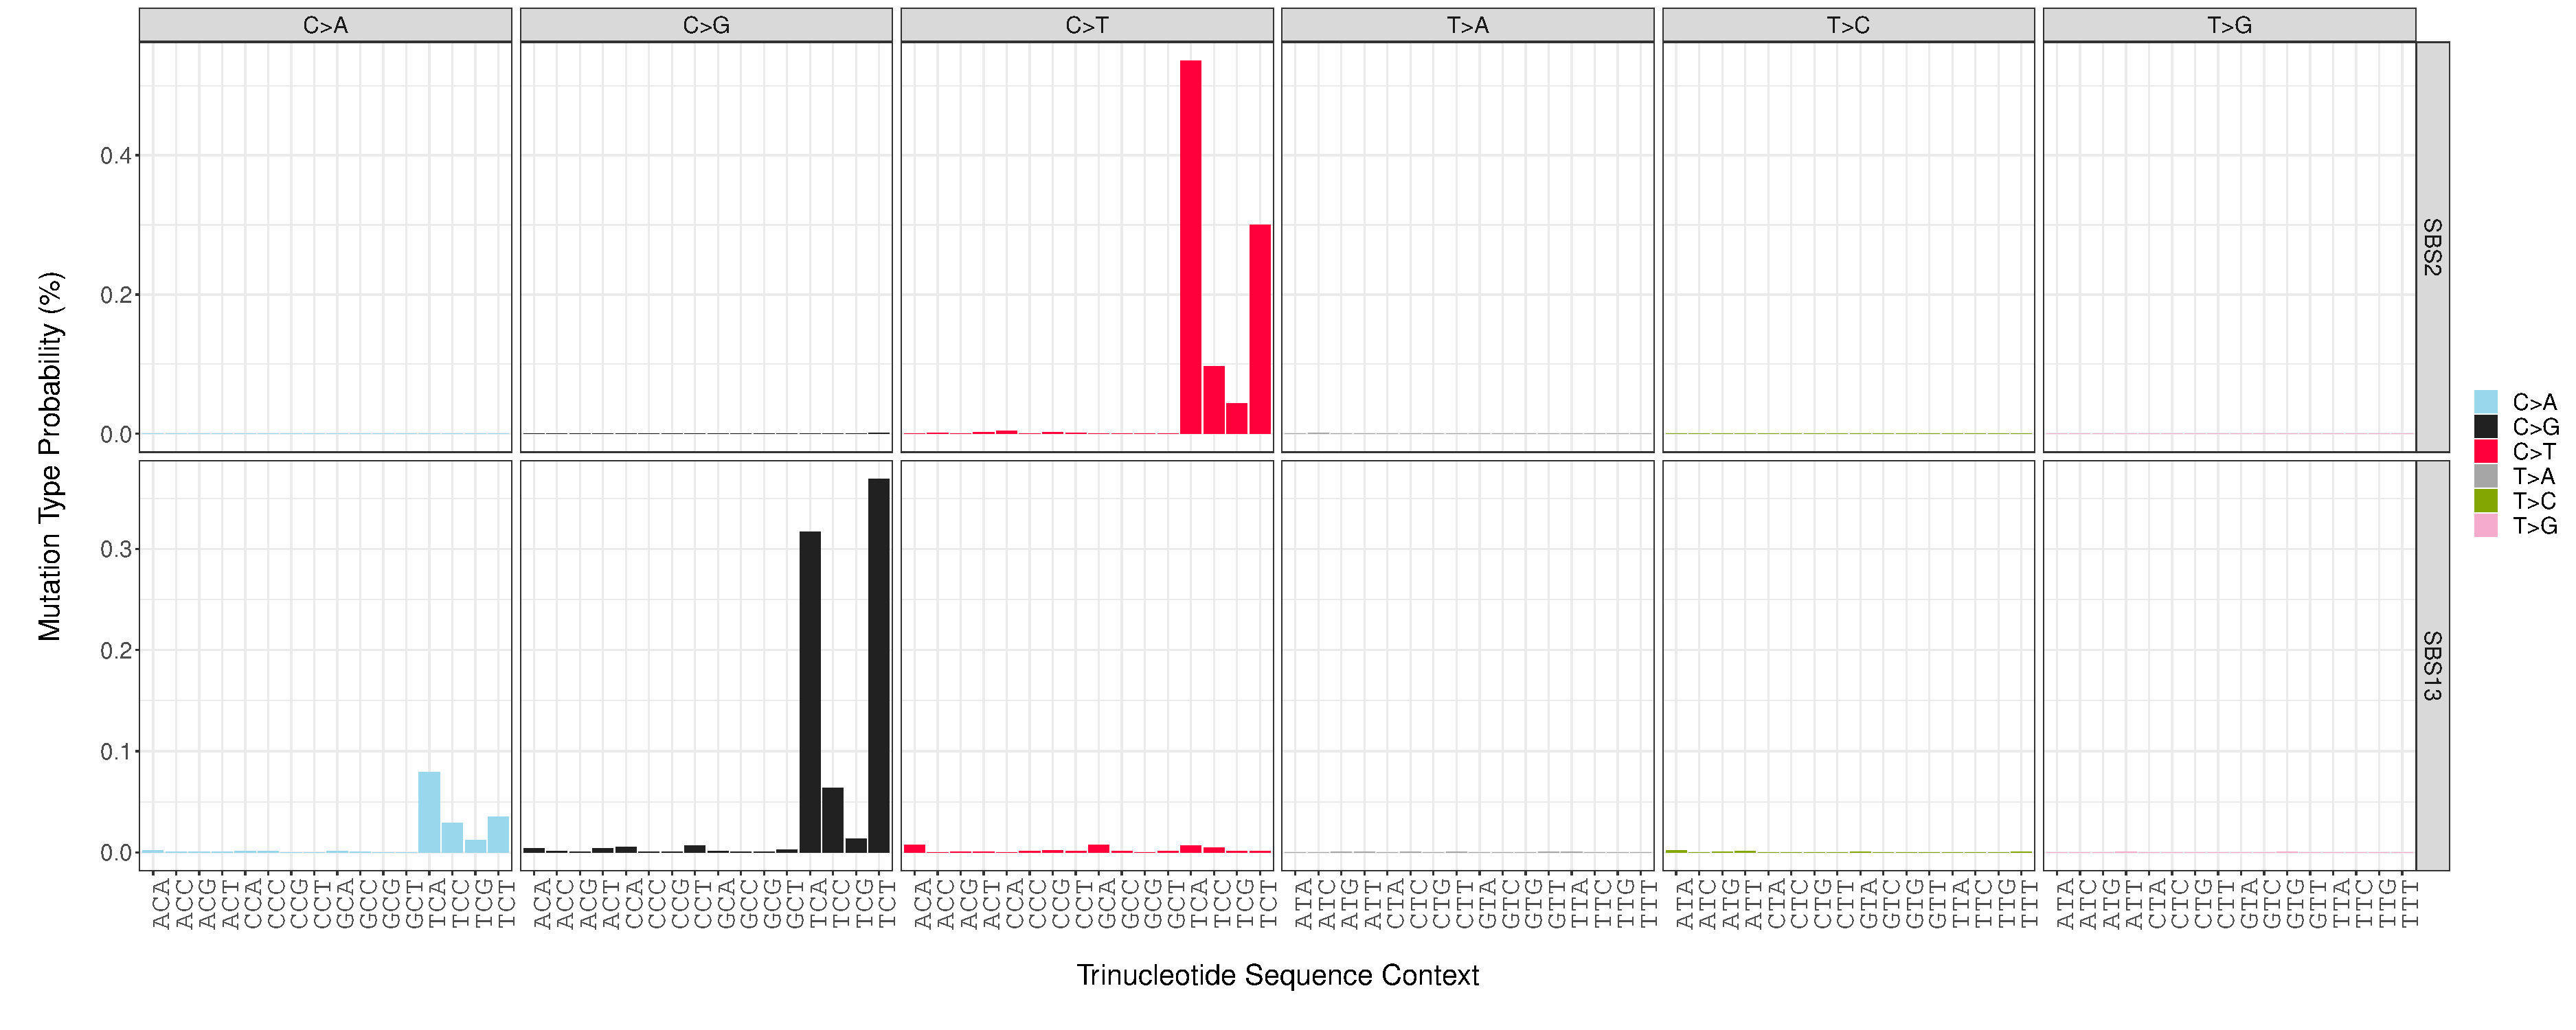
\includegraphics[width=1\textwidth]{Vector/SBS2_SBS13_sbs96.pdf}
\end{centering}
\end{figure}

During eukaryotic DNA replication, DNA polymerase $\delta$ (POLD) and $\varepsilon$ (POLE) are critical for DNA synthesis on the lagging and leading strand, respectively \cite{Swan2009-ew, Pursell2007-cu}. POLD and POLE enzymes both have intrinsic proofreading capabilities and their 3’-5’ exonuclease activity removes the 3’-terminal misincorporated nucleotide. Replicative DNA polymerases still introduce errors every $10^4 – 10^5$ nucleotides, but the mismatch repair (MMR) machinery corrects these errors. Individuals with inherited germline mutations or acquired somatic mutations that inactivate the POLE exonuclease activity have elevated somatic mutation rate and predisposes them to polymerase proofreading-associated polyposis, endometrial and colorectal cancers \cite{Palles2013-ua}. C>A mutations at TCN trinucleotides (SBS10a), C>A/C>T mutations at TCN trinucleotides (SBS10b) T>G mutations at NTT trinucleotides (SBS28) characterise POLE mutagenesis (Figure \ref{figure:pole-mutagenesis}) \cite{Robinson2021-te}. 

\begin{figure}[htbp!]
\caption{POLE mutagenesis}
\label{figure:pole-mutagenesis}
\begin{centering}
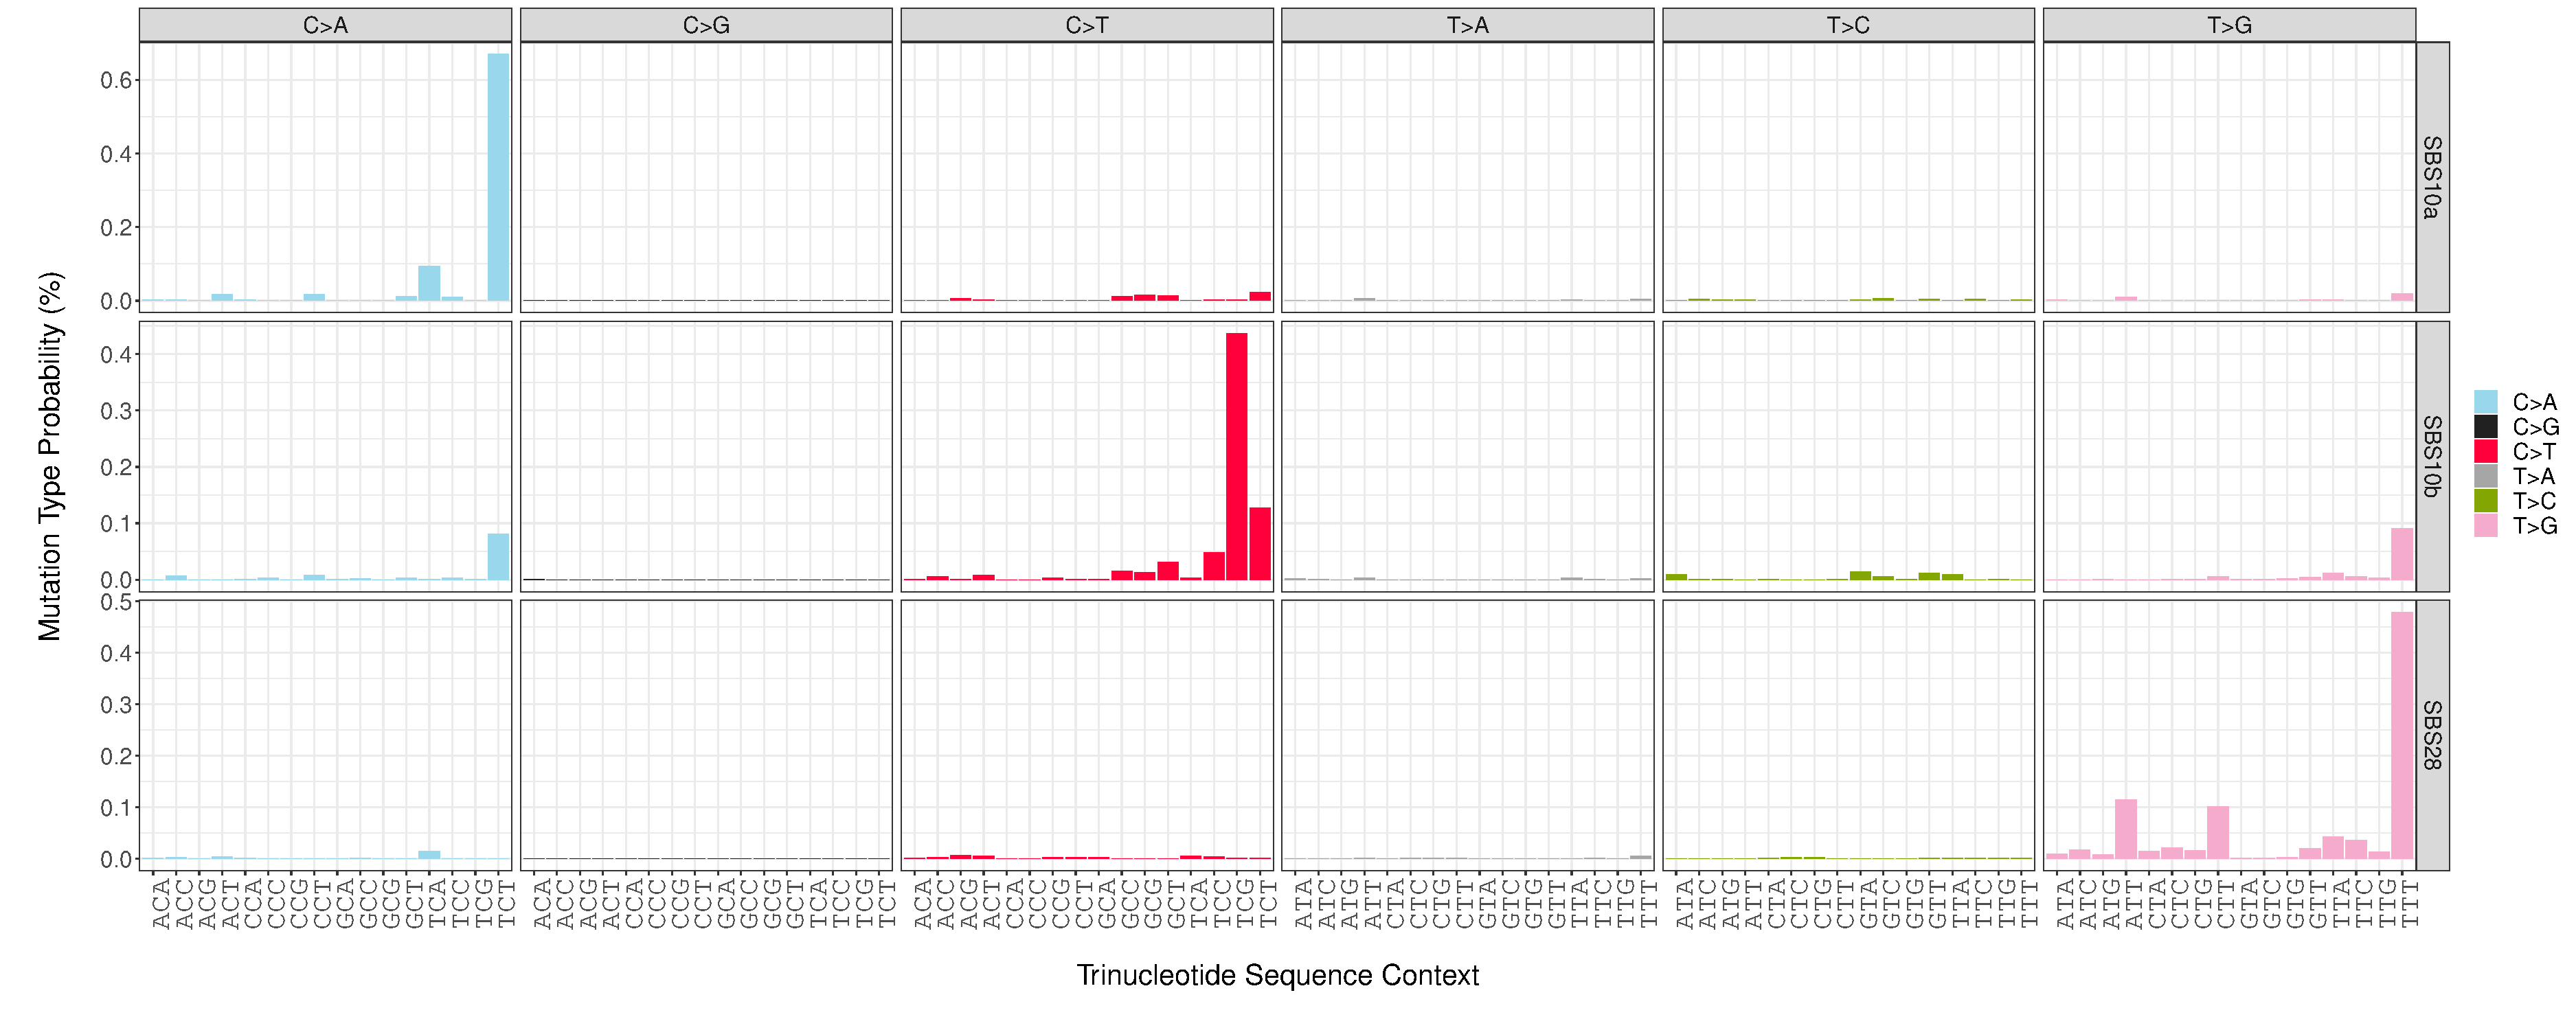
\includegraphics[width=\textwidth]{Vector/SBS10a_SBS10b_SBS28_sbs96.pdf}
\end{centering}
\end{figure}


Clock-like mutational processes are mutational processes that introduce somatic mutations at a constant rate throughout life and hence, the number of mutations attributable to clock-like mutational processes is proportional to the age of the individual. Clock-like mutational process is sample and species dependent, but C>T (SBS1) mutations at NCG trinucleotide and cell division independent mutational process (SBS5) (Figure \ref{figure:clock-like-mutagenesis}) are determined to be clock-like mutational processes in normal human tissues \cite{Alexandrov2015-db}. C>T mutations at CpG dinucleotide result from spontaneous deamination of 5-methylcytosine to thymine and the unrepaired T:G mismatch manifests as somatic mutations. The exact aetiology of SBS5 is unknown, but somatic mutagenesis study in post-mitotic tissues such as neurons and smooth muscle suggests that SBS5 might be a manifestation of multiple different cell division independent mutational processes \cite{Abascal2021-pk}.

\begin{figure}[htbp!]
\caption{Clock-like mutational processes}
\label{figure:clock-like-mutagenesis}
\begin{centering}
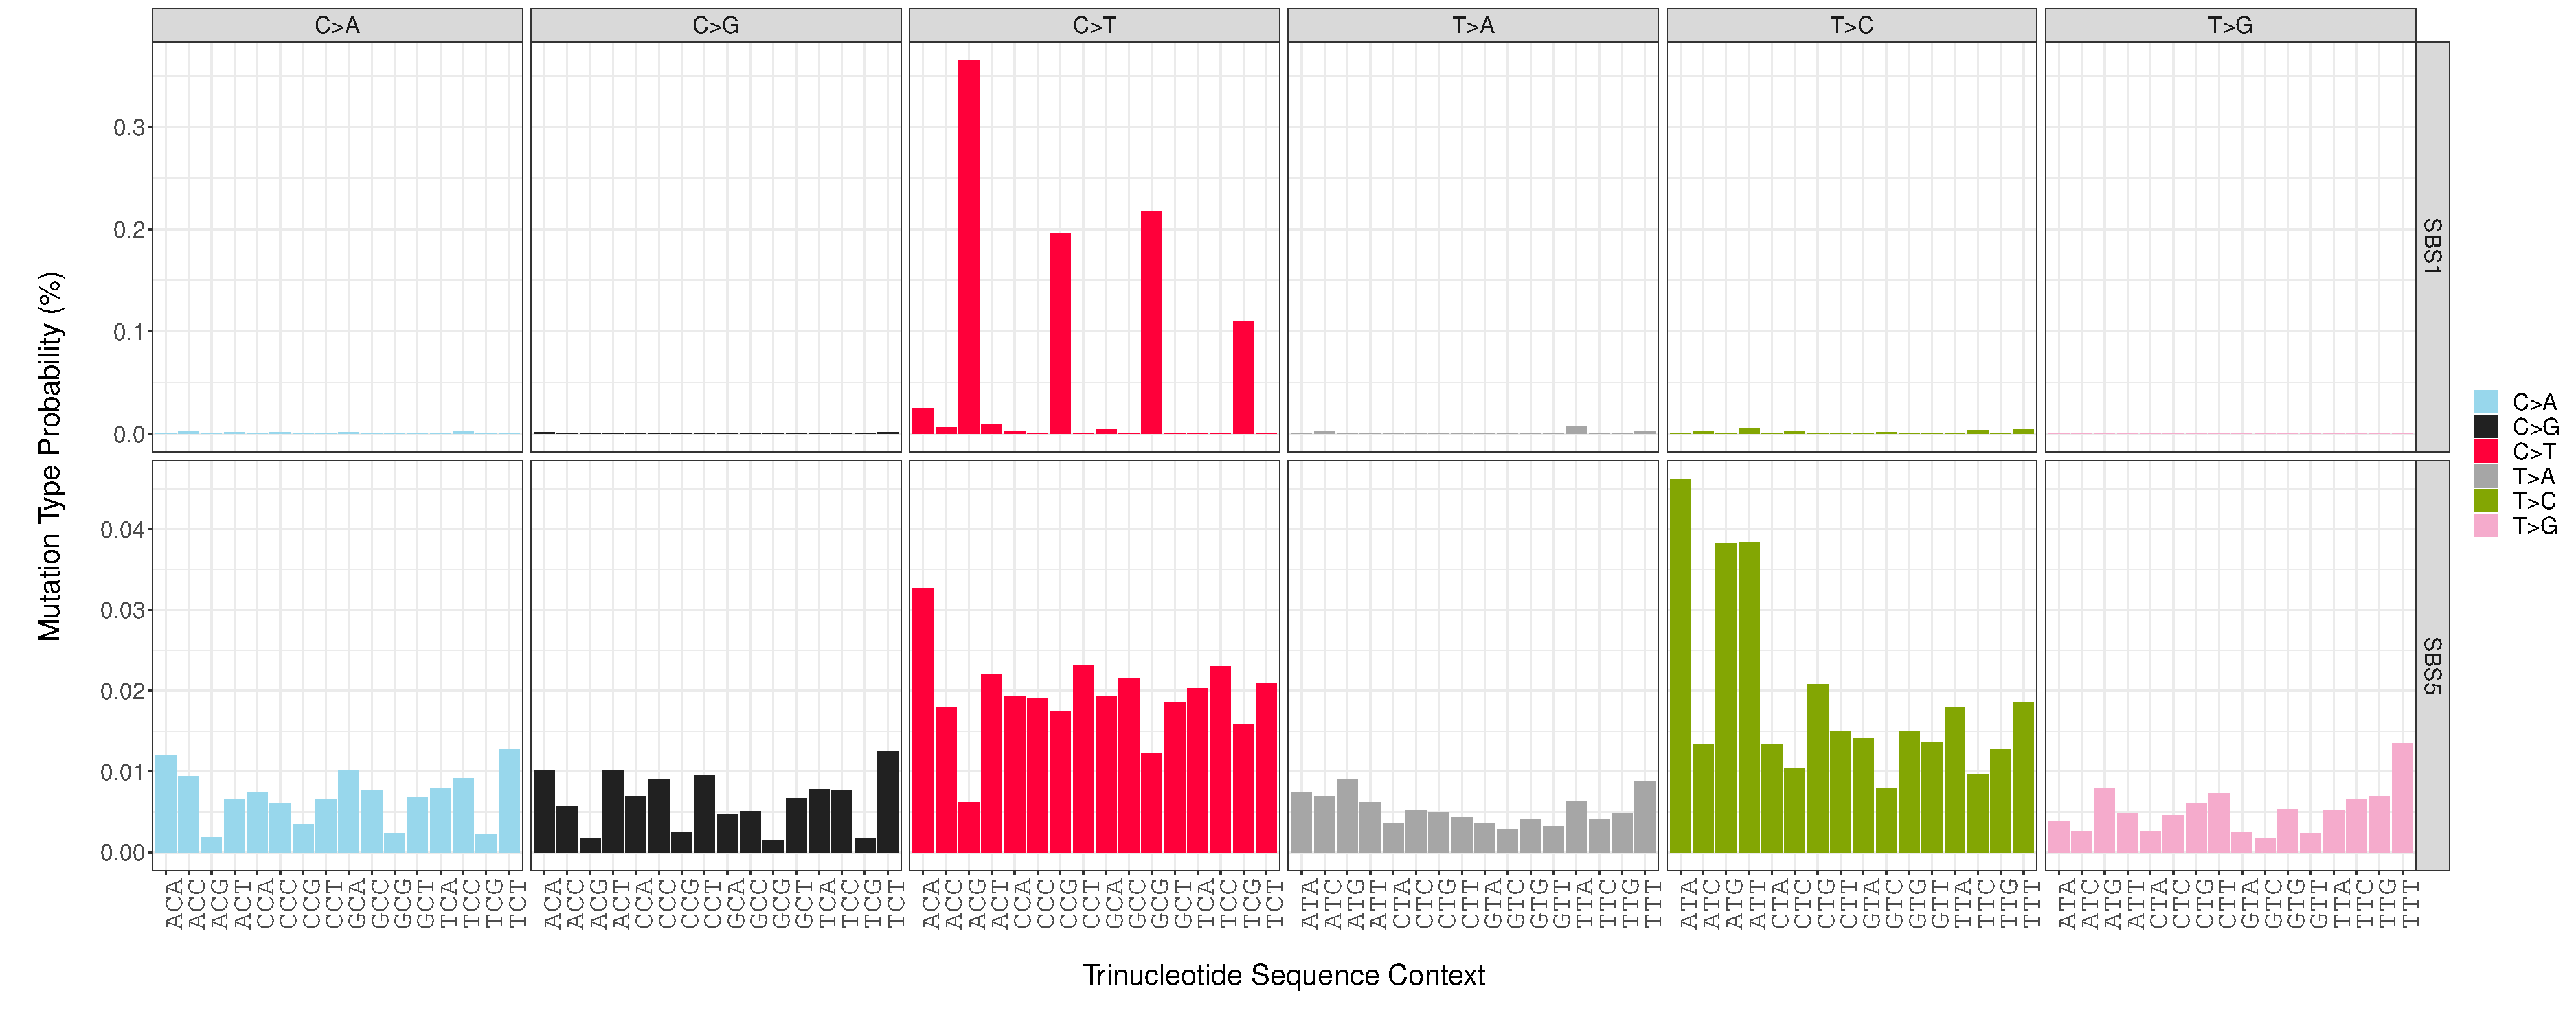
\includegraphics[width=\textwidth]{Vector/SBS1_SBS5_sbs96.pdf}
\end{centering}
\end{figure}

\pagebreak

\section{Results}

\subsection{CCS library errors and sequencing errors}

CCS reads have been successfully used for construction of highly contiguous and complete de novo assemblies \cite{Wenger2019-pw} and germline mutation detection \cite{Poplin2018-ub}. In these applications, the accuracy of individual base quality scores is not so important as ~50\% or ~100\% of the bases will support the consensus base, heterozygous or homozygous mutation. The accuracy of individual base quality scores, however, matters for ultra-rare somatic mutation detection as the base accuracy must be higher than the human genome somatic mutation rate to distinguish sequencing errors from single molecule somatic mutations (As discussed in the introduction, the human genome typically acquires somatic mutations at a rate between Q82 and Q93 per year, depending on the tissue). 

\begin{table}[h!]
\caption{Experimental Data}
\label{tab:CCS-sequence-statistics}
\begin{adjustbox}{max width=1.1\textwidth,center}
\begin{tabular}{l|cccc}
                                     & BC-1 & HT-115 & PD47269d & PD4873b \\ \hline
Genomic DNA source                   & \multicolumn{2}{c}{Cell line} & \multicolumn{2}{c}{Blood granulocyte} \\  \hline
Age (years)                 		 & - & - & 0 & 82  \\ \hline
CCS read count                       &  5,962,252 &  5,933,281 & 12,156,251 & 4,949,180 \\ \hline
Mean length $\pm$ std (bp)  & 18,571 $\pm$     & 17,038 $\pm$   &  16,523 $\pm$ 3,752 & 18,263 $\pm$ 1,753 \\ \hline
Q93 bases (\%) 						 & 51.4 & 55.5 & 57.6 & 51.7 \\ \hline
Sequence coverage 				     & 36.9 & 33.7 & 67.0 & 30.1 \\ \hline
Mutational process   			     & APOBEC & POLE & \multicolumn{2}{c}{Clock-like} \\ \hline
Mutational signature 				 & SBS2   & SBS10a, SBS10b and SBS28 & \multicolumn{2}{c}{SBS1 and SBS5} \\ \hline
Mutation burden per cell 		     & $\sim$2,000 - 22,000 & $\sim$8,000 - 11,000 & $\sim$40 - 50 & $\sim$1400 - 1500 \\ \hline 
\end{tabular}
\end{adjustbox} 
\floatfoot{CCS sequencing statistics, mutational process, associated mutational signatures and mutation burden are described for the negative control (PD47269d) and positive control (BC-1, HT-115 and PD48473b) samples.}
\end{table}

I generated 30-fold CCS sequence coverage from BC-1, HT-115 and blood granulocytes from an 82-year-old female individual (PD48473b) and 70-fold CCS sequence coverage from cord blood granulocyte (PD47269d) with an average read length between 16 and 20kb (Table \ref{tab:CCS-sequence-statistics}) to achieve the following objectives: 

\begin{enumerate}
\item to facilitate the design and development of a method (himut) for single molecule somatic mutation detection using CCS reads 
\item to empirically estimate the CCS error rate using CCS reads from cord blood granulocytes and to define the limit of detection threshold.
\item to evaluate himut sensitivity and specificity with changes in parameters.
\item to identify sources of errors and to develop solutions to reduce the contribution of errors to the total mutation burden of the sample
\end{enumerate}

I, first, analysed CCS and subreads from the same ZMW to identify false positive substitutions resulting from library and sequencing errors (Methods). I observed that 0.41-2.16\% of productive ZMWs have subreads arising from miscalling of adapter sequences (Table \ref{tab:adapter-miscalling-statistics}).

\begin{table}[h!]
\caption{Adapter miscalling statistics}
\label{tab:adapter-miscalling-statistics}
\begin{tabular}{c|c|c}
SMRTcell & Number of adapter miscalling & Number of productive ZMWs \\ \hline
m64089\_201022\_131119 & 2,696 (0.53\%) & 504,858 \\ \hline
m64089\_201023\_192624 & 2,222 (0.53\%) & 416,110 \\ \hline
m64089e\_210729\_164631 & 37,346 (2.00\%) & 1,867,538 \\ \hline
m64089e\_210731\_014247 & 41,723 (2.16\%) & 1,929,308 \\ \hline
m64089e\_210801\_075423 & 10,249 (1.27\%) & 804,082 \\ \hline
m64125\_201017\_124255 & 6,383 (0.41\%) & 1,539,077 \\ \hline
m64125\_201109\_000332 & 5,623 (0.45\%) & 1,241,983 \\ \hline
m64125\_201110\_063134 & 5,613 (0.44\%) & 1,282,810 \\ \hline
m64125e\_210718\_021224 & 29,351 (1.70\%) & 1,731,793 \\ \hline
m64125e\_210719\_111136 & 16,711 (1.84\%) & 909,397 \\ \hline
m64125e\_210720\_172316 & 5,452 (1.21\%) & 450,437 \\ \hline
\end{tabular}
\floatfoot{Adapter miscalling statistics from nine 8M SMRTcells used for PD47269 CCS sequencing}
\end{table}

I hypothesise that CCS reads with read length deviating from the mean CCS read length are the result of failed adapter sequence detection and exclude these CCS reads from somatic mutation detection (Method). In addition, I also noticed higher than expected adenine and thymine proportion and higher number of somatic mutations called from the end of CCS reads (Figure \ref{figure:base-proportion-per-ccs-position}). 

\begin{figure}[h!]
\caption{Base proportion per relative CCS position}
\label{figure:base-proportion-per-ccs-position}
\begin{centering}
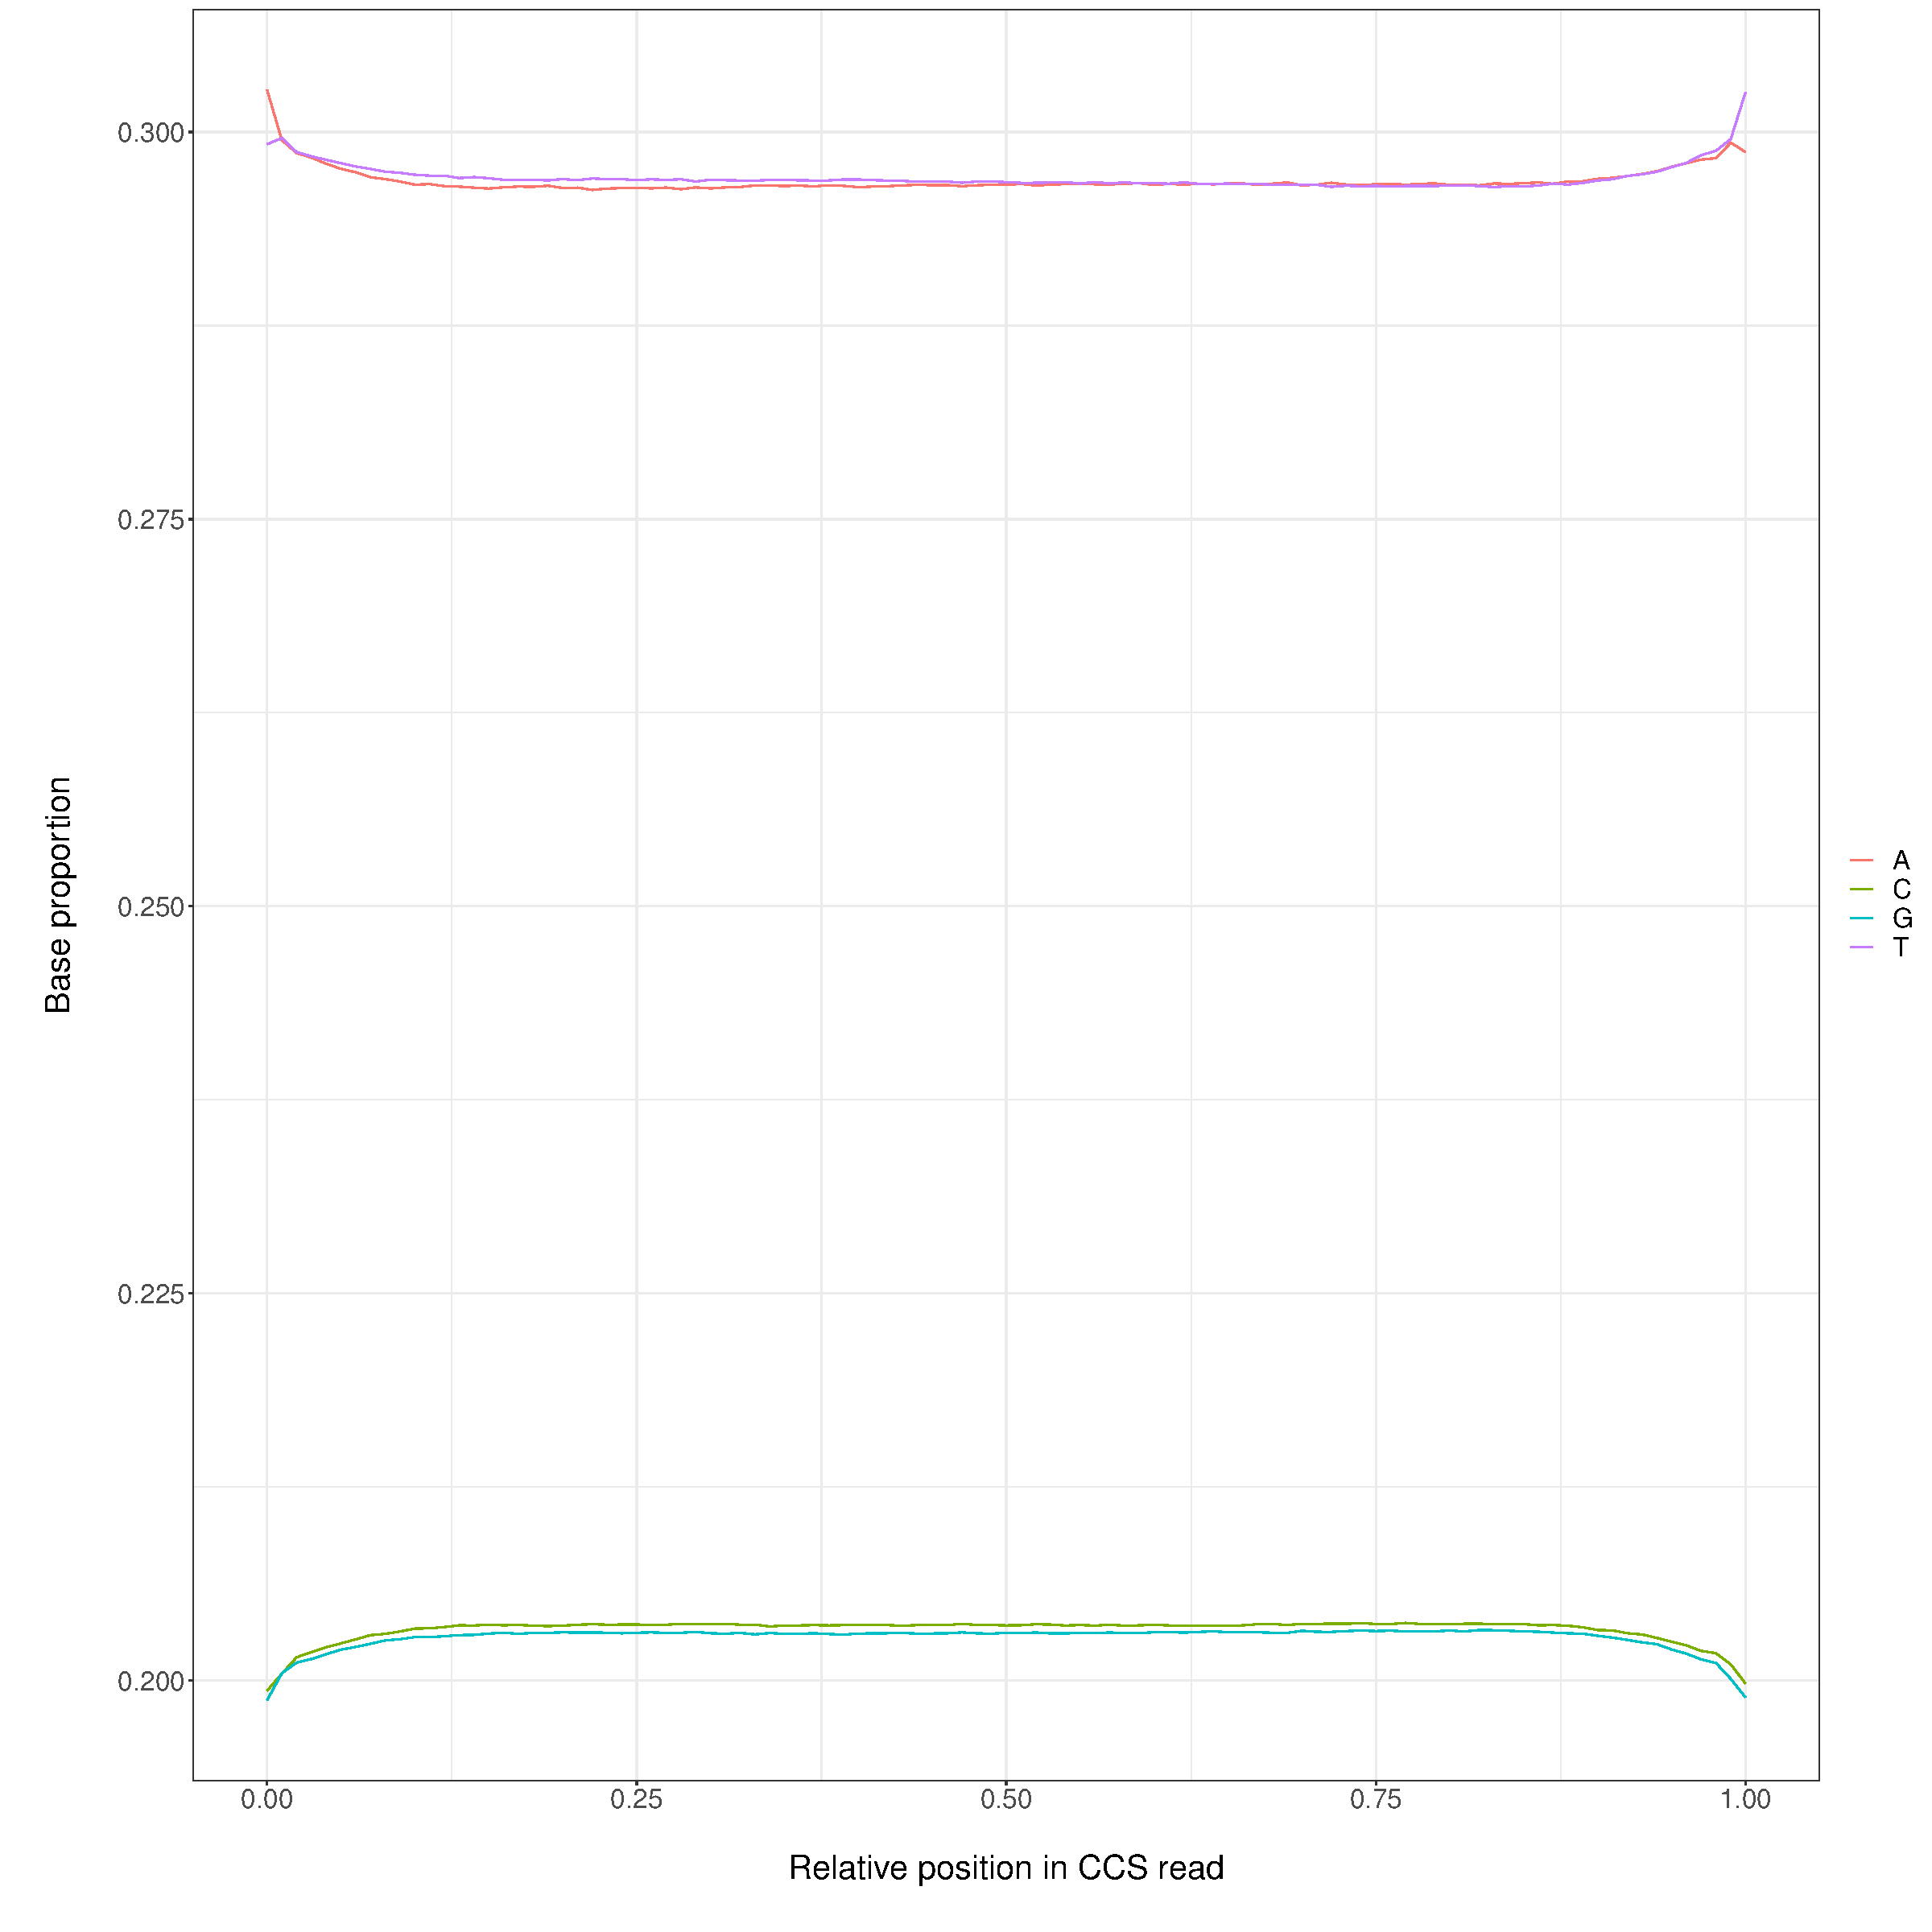
\includegraphics[width=0.6\textwidth]{Vector/base_proportion_per_ccs_position.pdf}
\end{centering}
\end{figure}

Incomplete adapter sequence trimming is thought to be responsible for this phenomenon. Hence, CCS reads with adapter sequences are removed before sequence alignment and somatic mutations called from 5’ and 3’ of CCS reads are discarded before downstream sequence analysis. 

CCS base BQ scores range from Q1 to nominal Q93, corresponding to $0.5\times10^{-9}$ error rate. A reduction in the number of mismatches to the reference genome is often used as a metric to evaluate whether CCS read generated from the more recent algorithm is superior to that produced from existing algorithms \cite{Wenger2019-pw, Baid2022-or}. This approach, however, discounts the presence of somatic mutations and assumes that all mismatches to the reference genome, that are not germline mutations, are errors. Here, I examined the accuracy of individual CCS base BQ score to assess the potential for single molecule somatic mutation detection using CCS reads (Figure \refP{})   

%\begin{figure}[htbp!]
%\caption{A boxplot of number of SBS per CCS read (sample: PD47269d)}
%\label{figure:sbs-count-per-ccs-read}
%\begin{centering}
%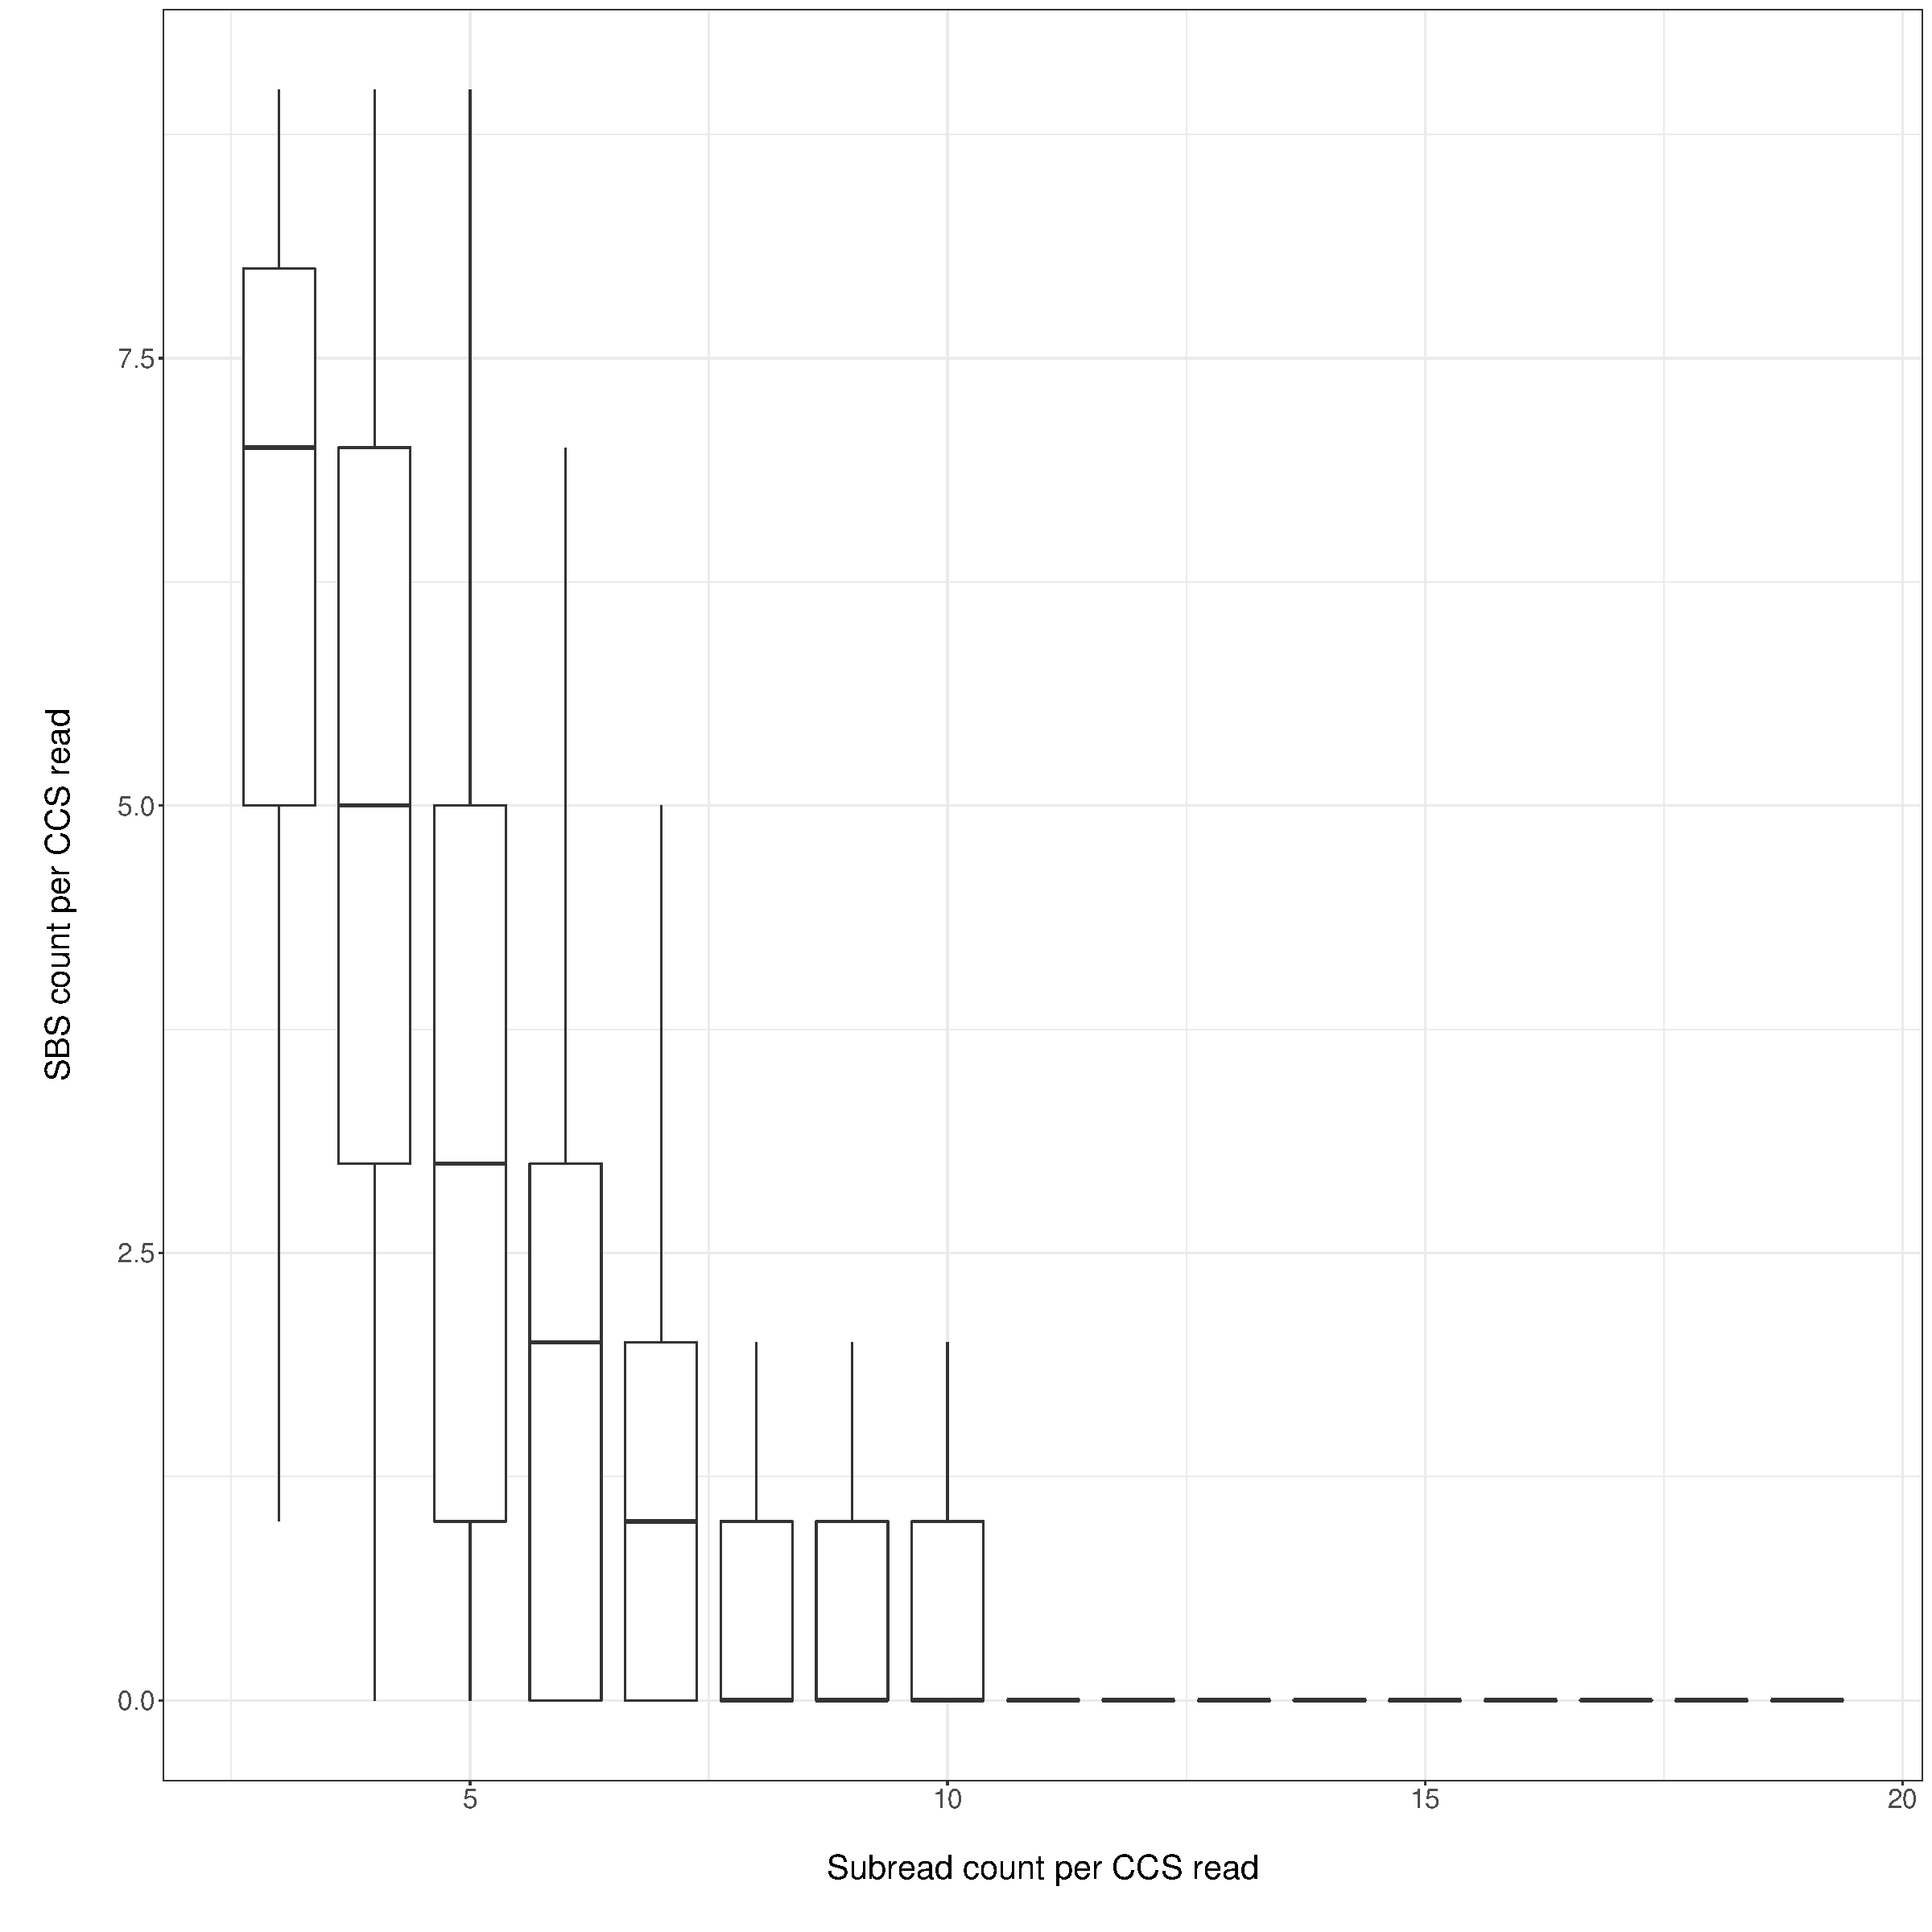
\includegraphics[width=0.6\textwidth]{Vector/sbs_count_per_ccs_read.pdf}
%\end{centering}
%\end{figure}

CCS BQ score is dependent on the number of subreads per CCS read and concordance between the subread bases and the CCS base. I was able to confirm that the number of substitutions and is negatively correlated with the number of subreads per CCS read as reported in a previous publication (Figure \ref{figure:sbs-count-per-ccs-read}) \cite{Wenger2019-pw}. 

\begin{figure}[htbp!]
\caption{A boxplot of number of SBS per CCS read (sample: PD47269d)}
\label{figure:sbs-count-per-ccs-read}
\begin{centering}
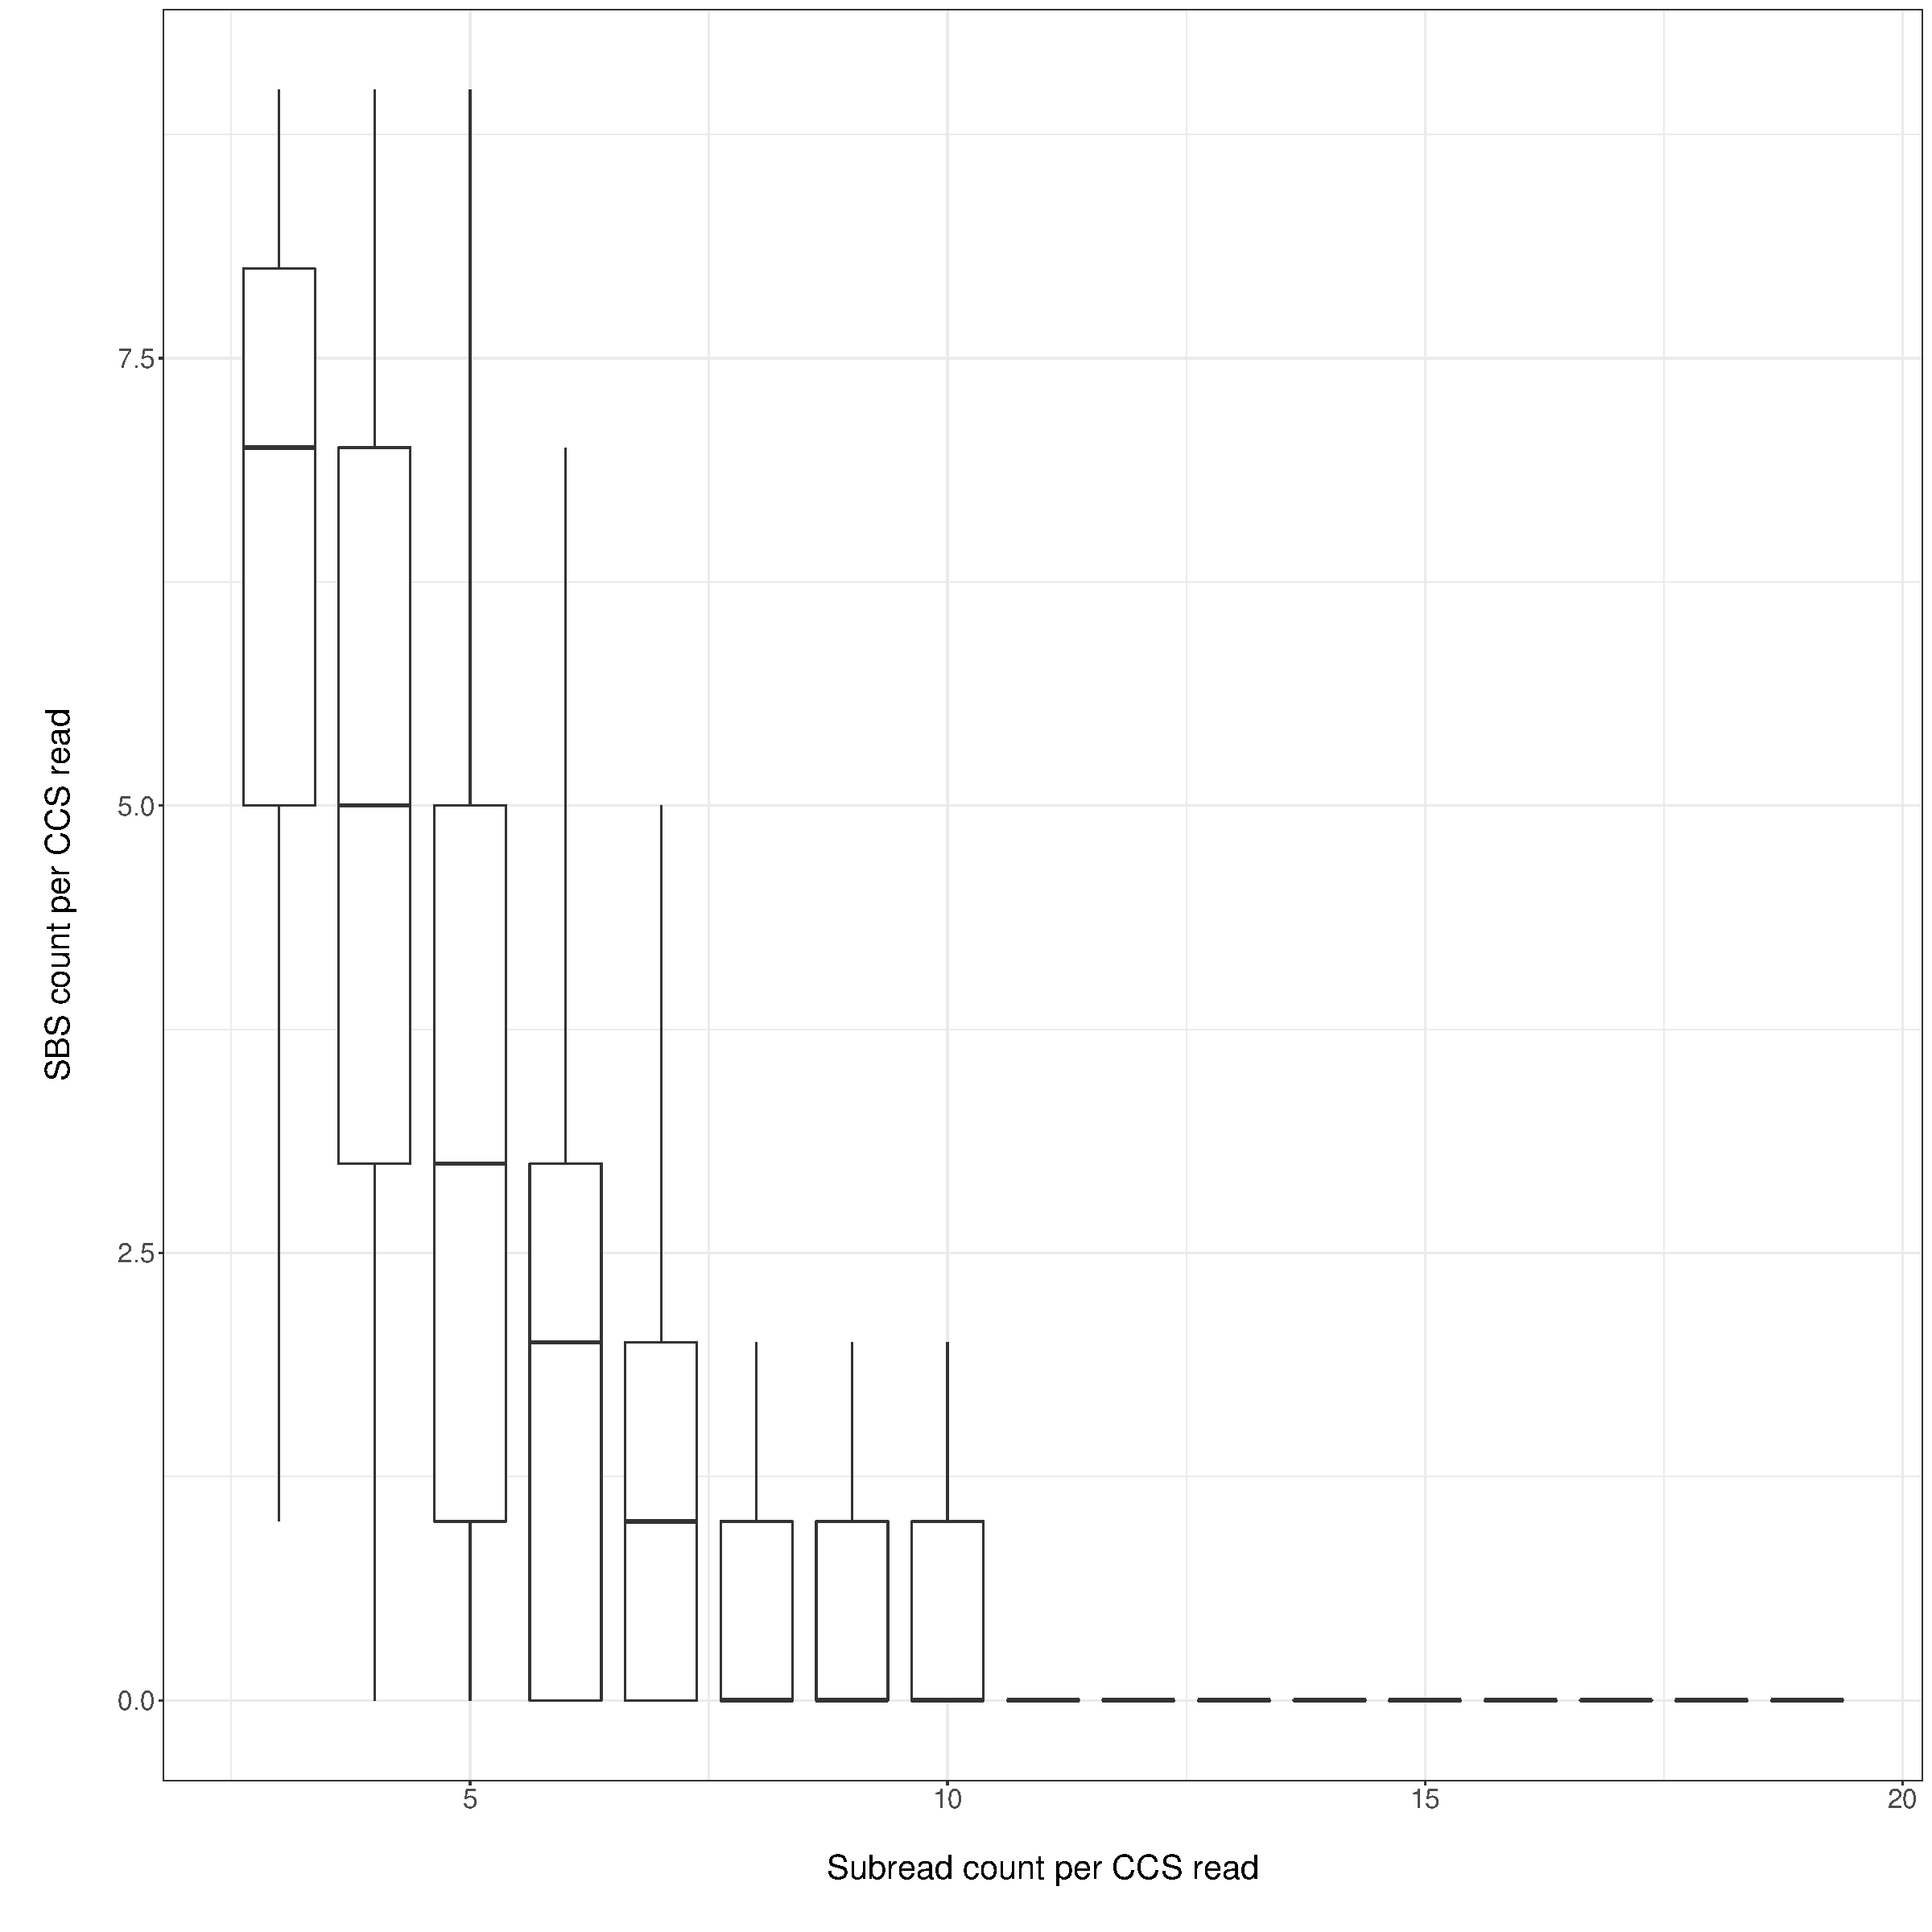
\includegraphics[width=0.6\textwidth]{Vector/sbs_count_per_ccs_read.pdf}
\end{centering}
\end{figure}

The accuracy of the BQ score, hence, is expected to increase with the number of supporting subread bases. I, however, discovered that the accuracy of the CCS BQ score decreases with increase in the number of subreads and that increase in the number of subreads per CCS read results in not diminishing returns, but negative returns to CCS base accuracy (discussed later in Chapter 3). 

Despite these issues, I was able to demonstrate that CCS read have sufficient base accuracy for single molecule somatic mutation in most normal human tissue. Firstly, I used the positive control samples to identify and evaluate parameters that influence somatic mutation detection sensitivity and specificity. Secondly, I used the negative control sample to determine the CCS error rate for Q93 CCS bases and the limit of detection threshold. Finally, I was able to find potential solutions to minimise the number of false positive mutations arising from errors upstream of downstream sequence analysis. 


\subsection{Germline mutation detection}

Bulk normal tissue has germline mutations that are inherited from parents, mosaic mutations that occurred during embryonic development and newly acquired somatic mutations from ongoing mutational processes. In addition, cells with driver mutations can outcompete neighbouring cells and clones of cells can occupy pockets of tissues. These clonal somatic mutations can often be confused with heterozygous germline mutations in normal bulk tissue. To distinguish germline mutations from somatic mutations, paired tumour-normal sequencing is often performed. In contrast, himut can confidently call somatic mutations from a bulk tissue without a matched normal sample (Methods). 

I, first, compared germline SNPs detected from both himut and deepvariant to assess whether our algorithm can accurately call germline mutations (Methods, Table \ref{}).

\begin{table}[h!]
\caption{Germline mutation statistics (sample: PD47269d)}
\label{tab:adapter-miscalling-statistics}
\begin{tabular}{c|c|c}
& Deepvariant & Himut \\ \hline
Heterozygous SNP & 2,394,488 & 2,040,007 \\ \hline
Homozygous SNP & 1,493,950 & 1,292,806 \\ \hline
TiTv ratio & 2.00 & 2.08 \\ \hline
\end{tabular}
\end{table}

The number of SNPs and transition to transversion (TiTv) ratio is within the expected range, demonstrating that himut can also function as a standalone variant caller. Deepvariant is a deep learning method that uses uses read pileup images for germline mutation detection. On the other hand, himut uses an analytical approach like GATK and strelka2 \cite{Kim2018-qi, DePristo2011-vf}  for germline mutation detection. Here, the germline mutation detected using himut is restricted to that with GQ score above 20, while that from deepvariant is not filtered.

\subsection{Somatic mutation detection}

To distinguish germline mutations from somatic mutations, himut first collects single-base-substitution (SBS) candidates from CCS reads that meets the read-level prerequisites (Methods). Afterwards, SBS candidates are classified as either a germline mutation or as co-occurrence of both germline and somatic mutation. Germline mutation is further categorised as a heterozygous, heterozygous alternative (tri-allelic), homozygous alternative or homozygous reference allele (Methods). Somatic mutation candidates occurring on heterozygous, heterozygous alternative or homozygous alternative alleles are labelled as somatic reversions and are not considered further as somatic reversions can also arise from gDNA contamination. To be classified as a somatic mutation, somatic mutation candidate must originate from a homozygous reference allele site and fulfil several base-level prerequisites that distinguishes mutations from errors (Methods, Figure \ref{figure:somatic-mutation-detection}). A VCF file with common SNPs and a PoN VCF file can also be optionally provided to exclude false positive mutations resulting from DNA contamination and systematic errors, respectively. Afterwards, himut calculates the mutation burden of the sample based on the number of called somatic mutations and the number of callable CCS and reference base (Methods). 

\begin{figure}[htbp!]
\caption{A framework for single molecule somatic mutation detection using himut}
\label{figure:somatic-mutation-detection}
\begin{centering}
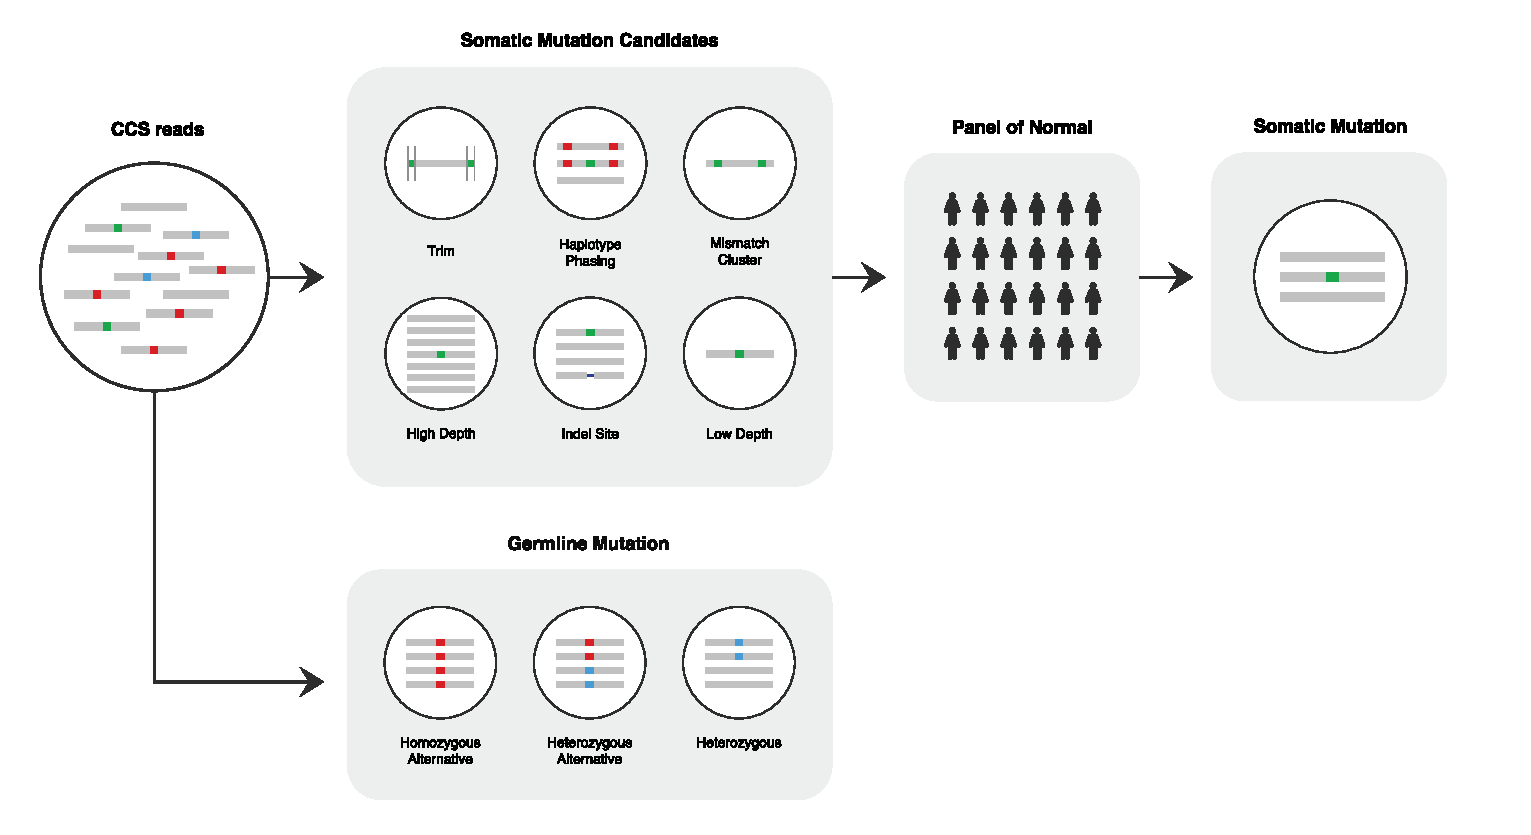
\includegraphics[width=\textwidth]{Vector/himut.pdf}
\end{centering}
\floatfoot{Red and blue rectangle indicates germline mutations while green rectangle indicates either somatic mutation candidates or called somatic mutations. After selection of CCS reads that meets pre-defined thresholds, a SBS is defined either as a germline mutation or as a somatic mutation candidate. Afterwards, a number of hard filters are applied to the somatic mutation candidate to determine whether it is an error or a somatic mutation. A PoN VCF can be optionally supplied to filter false positive somatic mutations arising from systematic errors.}
\end{figure}

\pagebreak

\subsubsection{Haplotype phased somatic mutation detection}

If a sample has a low sequence coverage, himut can also leverage CCS read length and base accuracy to phase heterozygous SNPs (hetSNPs) and connect phased hetSNPs to construct contiguous haplotype blocks (Methods). A VCF file containing haplotype phased hetSNPs to identify genomic regions where both haplotypes of the diploid genome have been sampled sufficiently and to call haplotype phased somatic mutations (Methods), which has numerous advantages to read-backed phasing of somatic mutations with Illumina reads (Figure \ref{figure:haplotype-phased-somatic-mutation-detection}).

\begin{enumerate}
\item Read-backed phasing with Illumina reads uses adjacent hetSNPs to phase approximately $\sim$30\% of detected somatic mutations \cite{Nik-Zainal2012-nz}. In contrast, haplotype phased somatic mutation detection with CCS reads uses all hetSNPs that the CCS read spans and phases approximately $\sim$70\% of somatic mutations.
\item CCS reads derived from gDNA contamination often have a different haplotype than that of the sample. Consequently, if haplotype of a CCS read does not match the consensus haplotype of the sample, it can be classified as a contamination and be excluded from analysis.
\item If somatic mutation detection is restricted to haplotype phased regions, hetSNP cannot be misclassified as a somatic mutation as haplotype phasing requires sufficient sampling of both haplotypes.
\item CCS reads with the same somatic mutation should share the same haplotype. If a somatic mutation should is present on both haplotypes, it can be categorised as an error.
\end{enumerate}

\begin{figure}[htbp!]
\caption{A framework for haplotype phased somatic mutation detection}
\label{figure:haplotype-phased-somatic-mutation-detection}
\begin{centering}
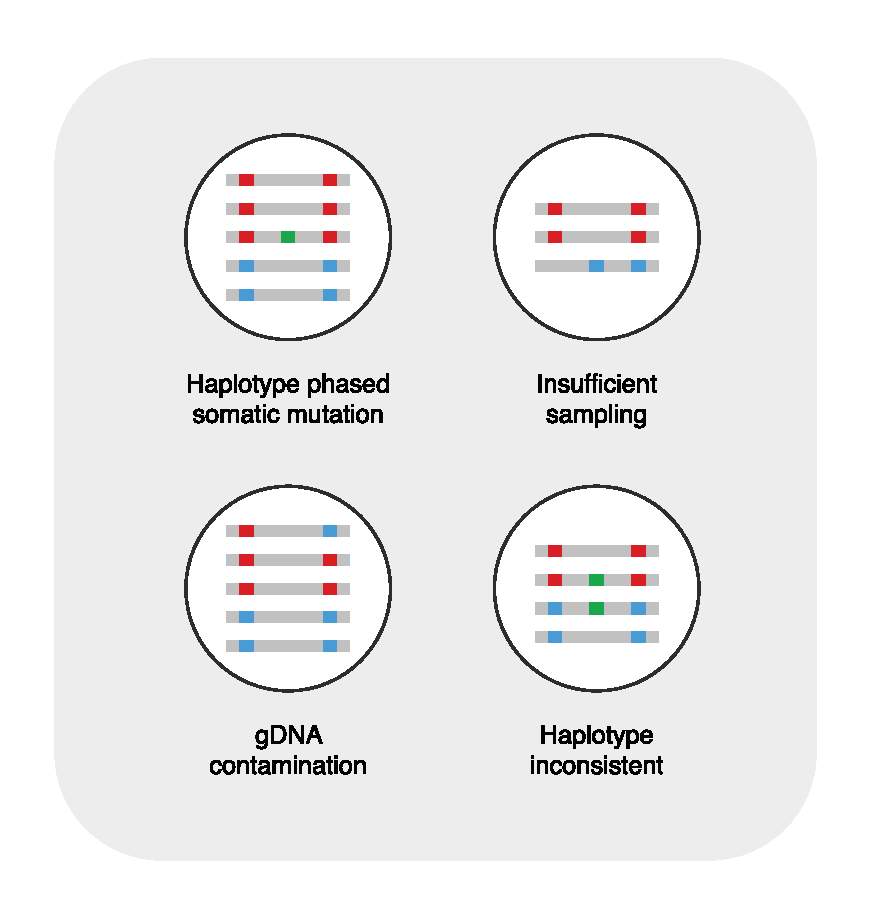
\includegraphics[width=\textwidth]{Vector/haplotype_phased_somatic_mutation_detection.pdf}
\end{centering}
\floatfoot{As before, red and blue rectangle indicates germline mutations while green rectangle indicates either somatic mutation candidates or called somatic mutations. }
\end{figure}

\subsection{Somatic mutation detection sensitivity and specificity}

I called and benchmarked haplotype unphased and phased somatic mutations from the three positive controls with different mutational burdens and distinct mutational processes. Our unique benchmarking approach leverages the fact that a single somatic mutational process is active in each sample and that somatic mutation candidates are derived from either errors or newly acquired somatic mutations. Himut cannot be certain whether individual somatic mutations are derived from an error or a somatic mutational process, but if there is sufficient signal-to-noise ratio, mutational spectrum produced from the aggregate somatic mutations should be consistent with the expected mutational signature. In addition, our approach is not biased towards Illumina callable regions of the genome unlike the Genome in a Bottle (GIAB) benchmarks \cite{Zook2014-et} as our somatic mutation detection method is agnostic to reference position. 

The mutational spectrum generated from BC-1 (Figure \ref{figure:BC-1}), HT-115 (Figure \ref{figure:HT-115}) and PD48473b (Figure \ref{figure:PD48473b}) somatic mutations were concordant with the expected mutational signatures from these samples (Methods). 

\begin{figure}[htbp!]
\caption{Comparison between SBS2 and the BC-1 mutational spectrum}
\label{figure:BC-1}
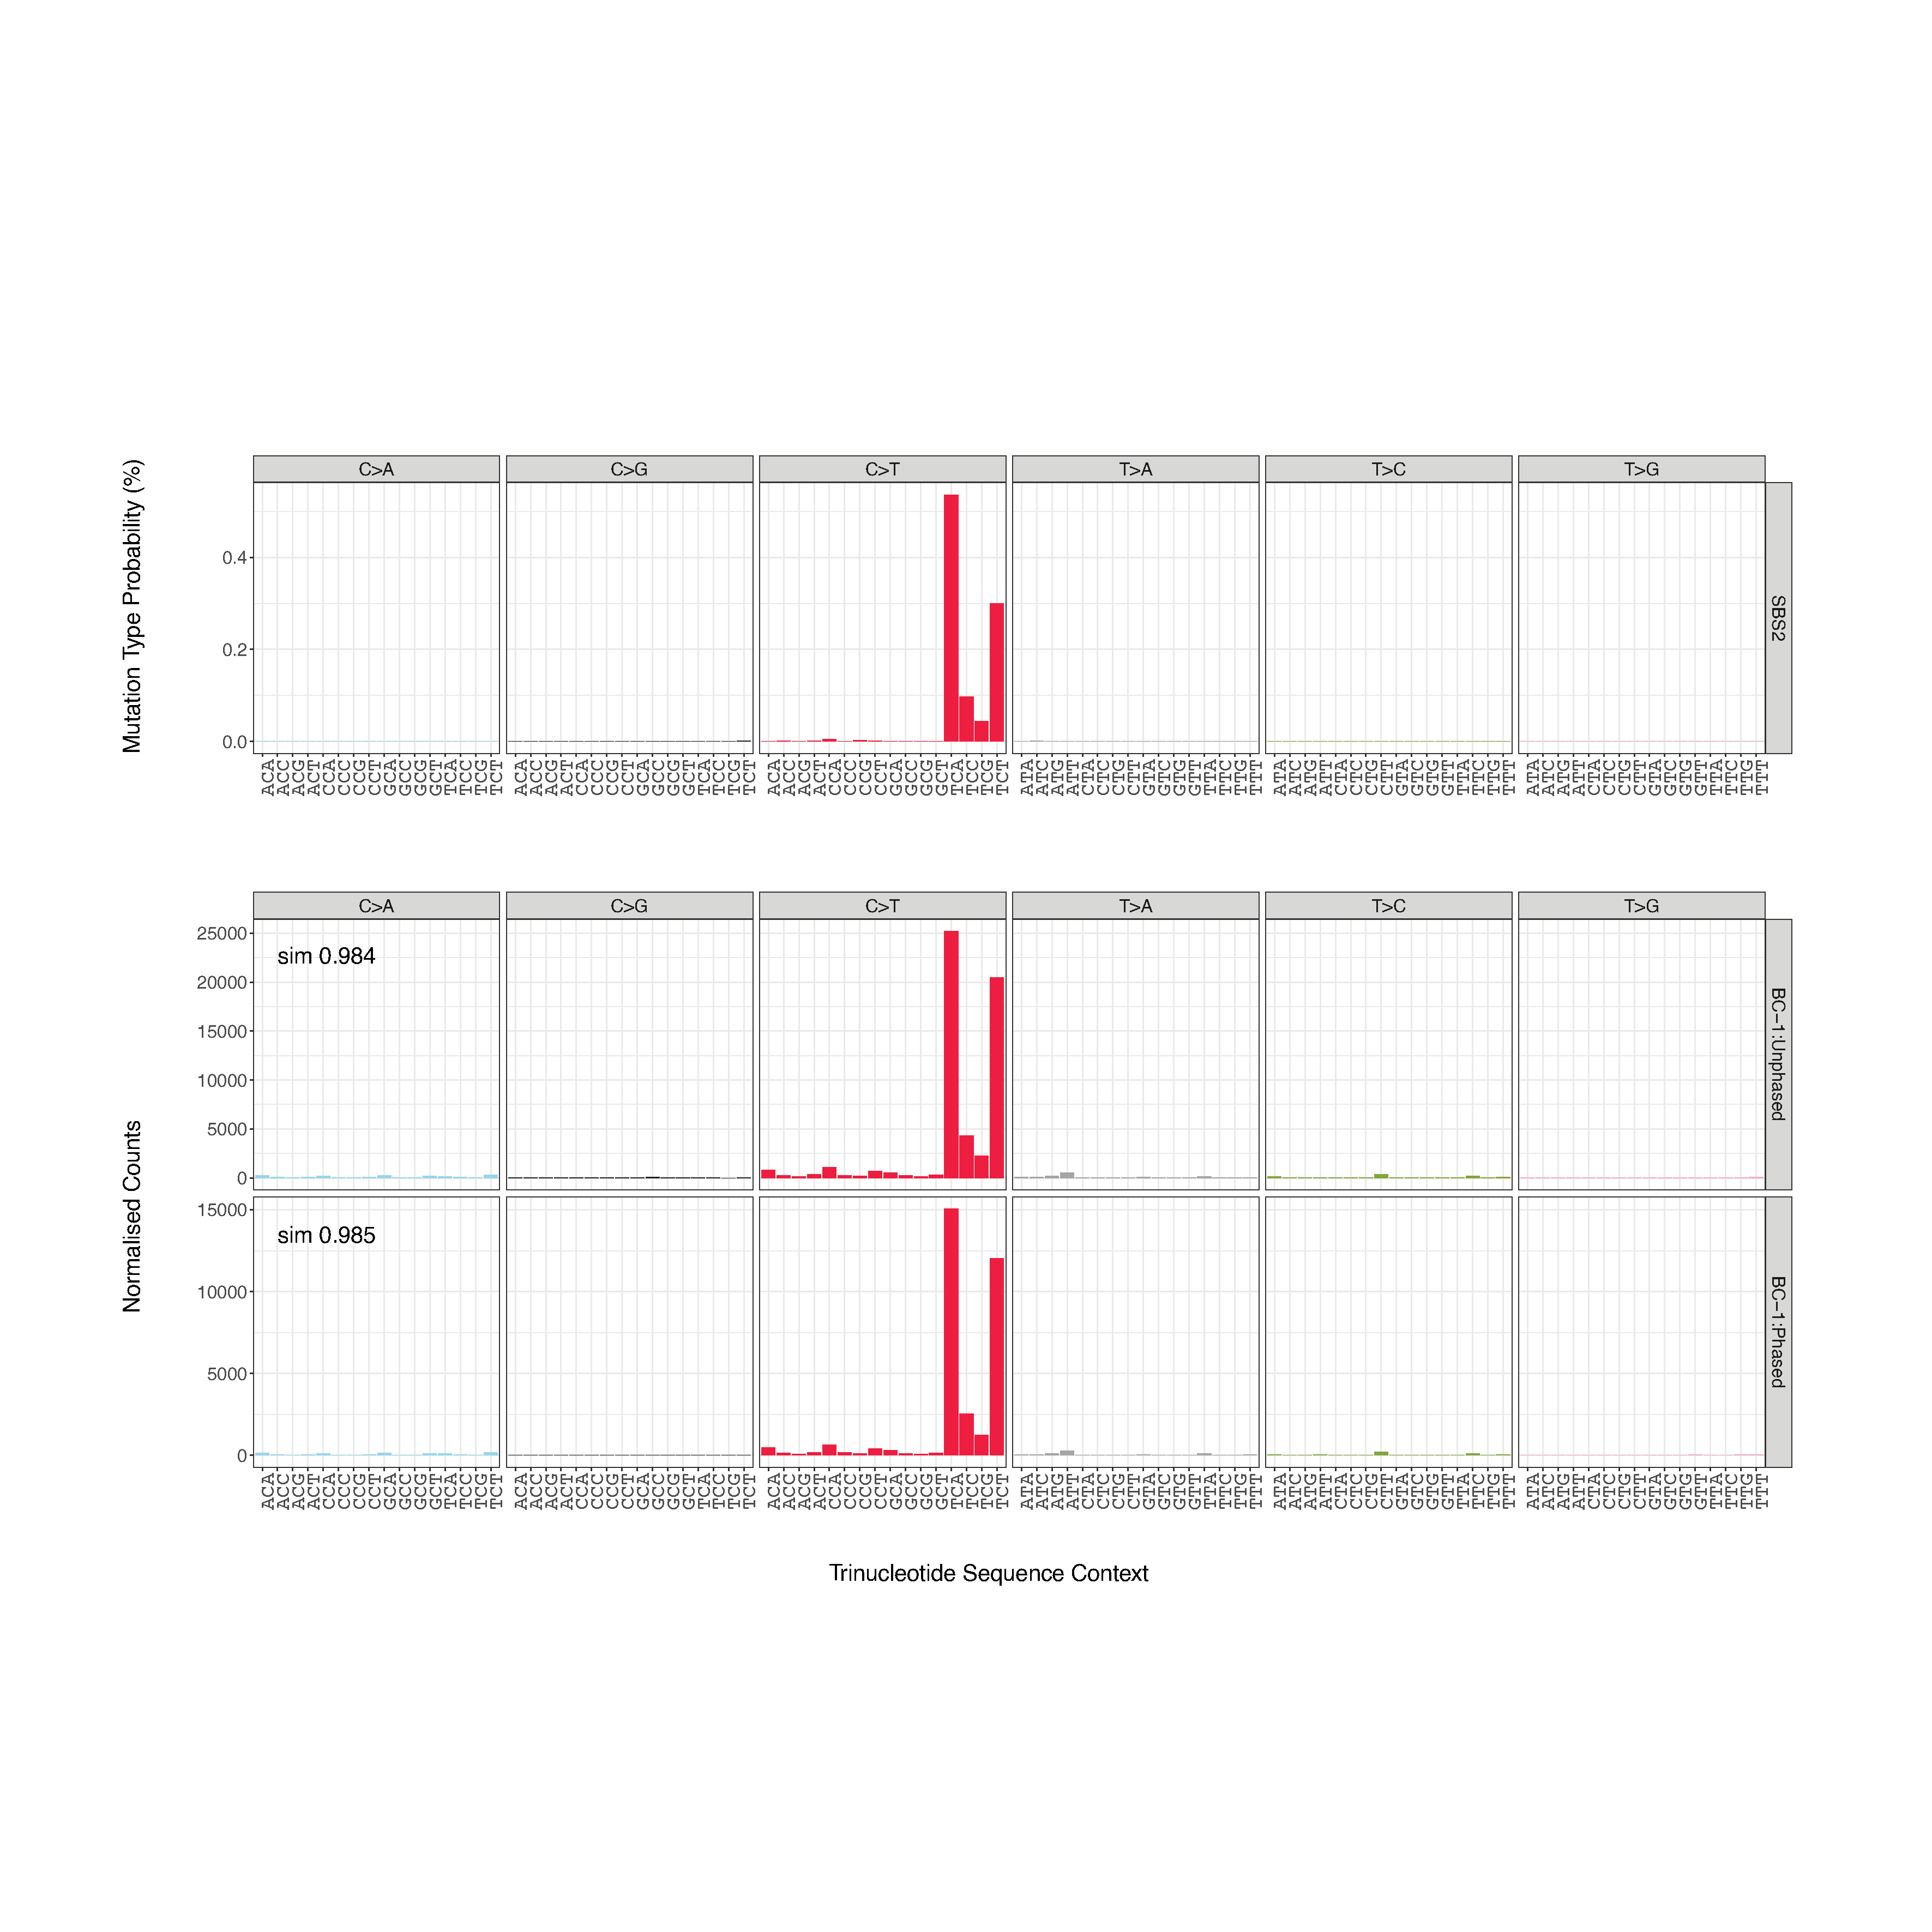
\includegraphics[width=\textwidth]{Vector/hg19.SBS2.BC-1.pdf}
\end{figure}

\begin{figure}[htbp!]
\caption{Comparison between the linear combination of SBS10a, SBS10b and SBS28 and the HT-115 mutational spectrum}
\label{figure:HT-115}
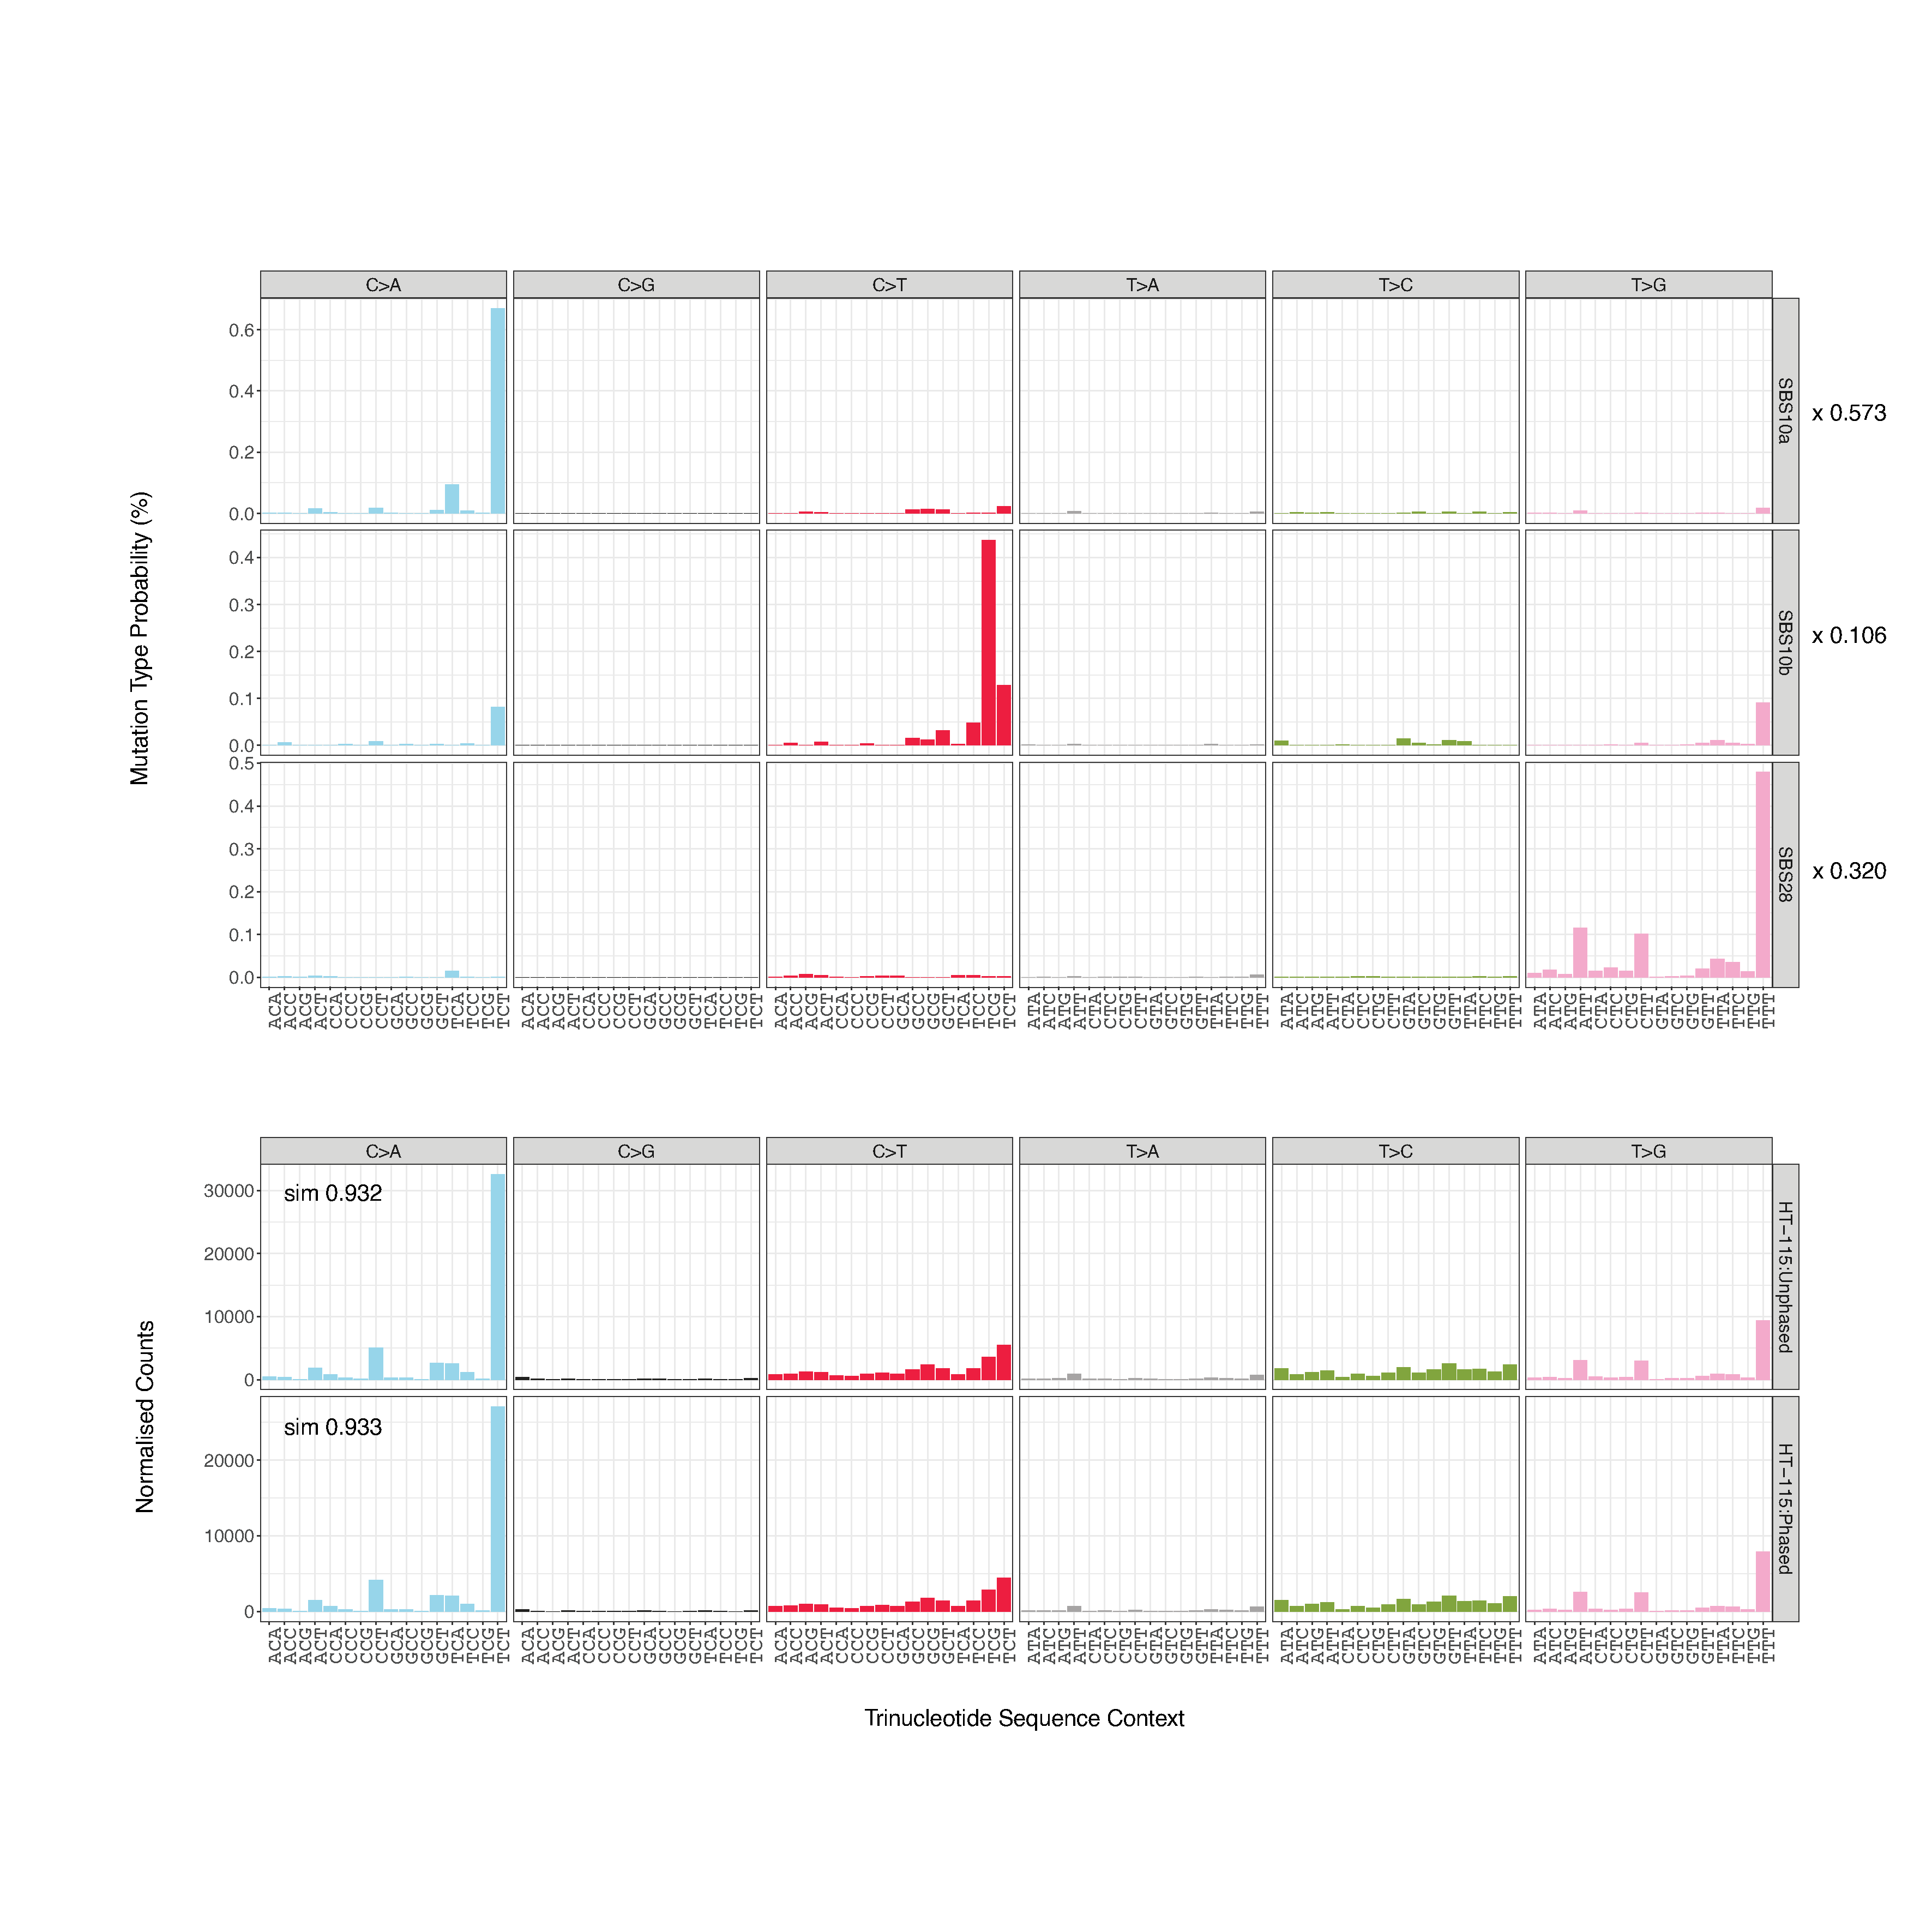
\includegraphics[width=\textwidth]{Vector/hg19.SBS10a.SBS10b.SBS28.HT-115.pdf}
\floatfoot{As previously observed \cite{Petljak2019-wi}, the contribution of SBS10b to the mutational burden of the HT-115 sample is reduced in \textit{in vitro} conditions.}
\end{figure}

\begin{figure}[htbp!]
\caption{Comparison between KX004 mutational spectrum and the PD48473b mutational spectrum}
\label{figure:PD48473b}
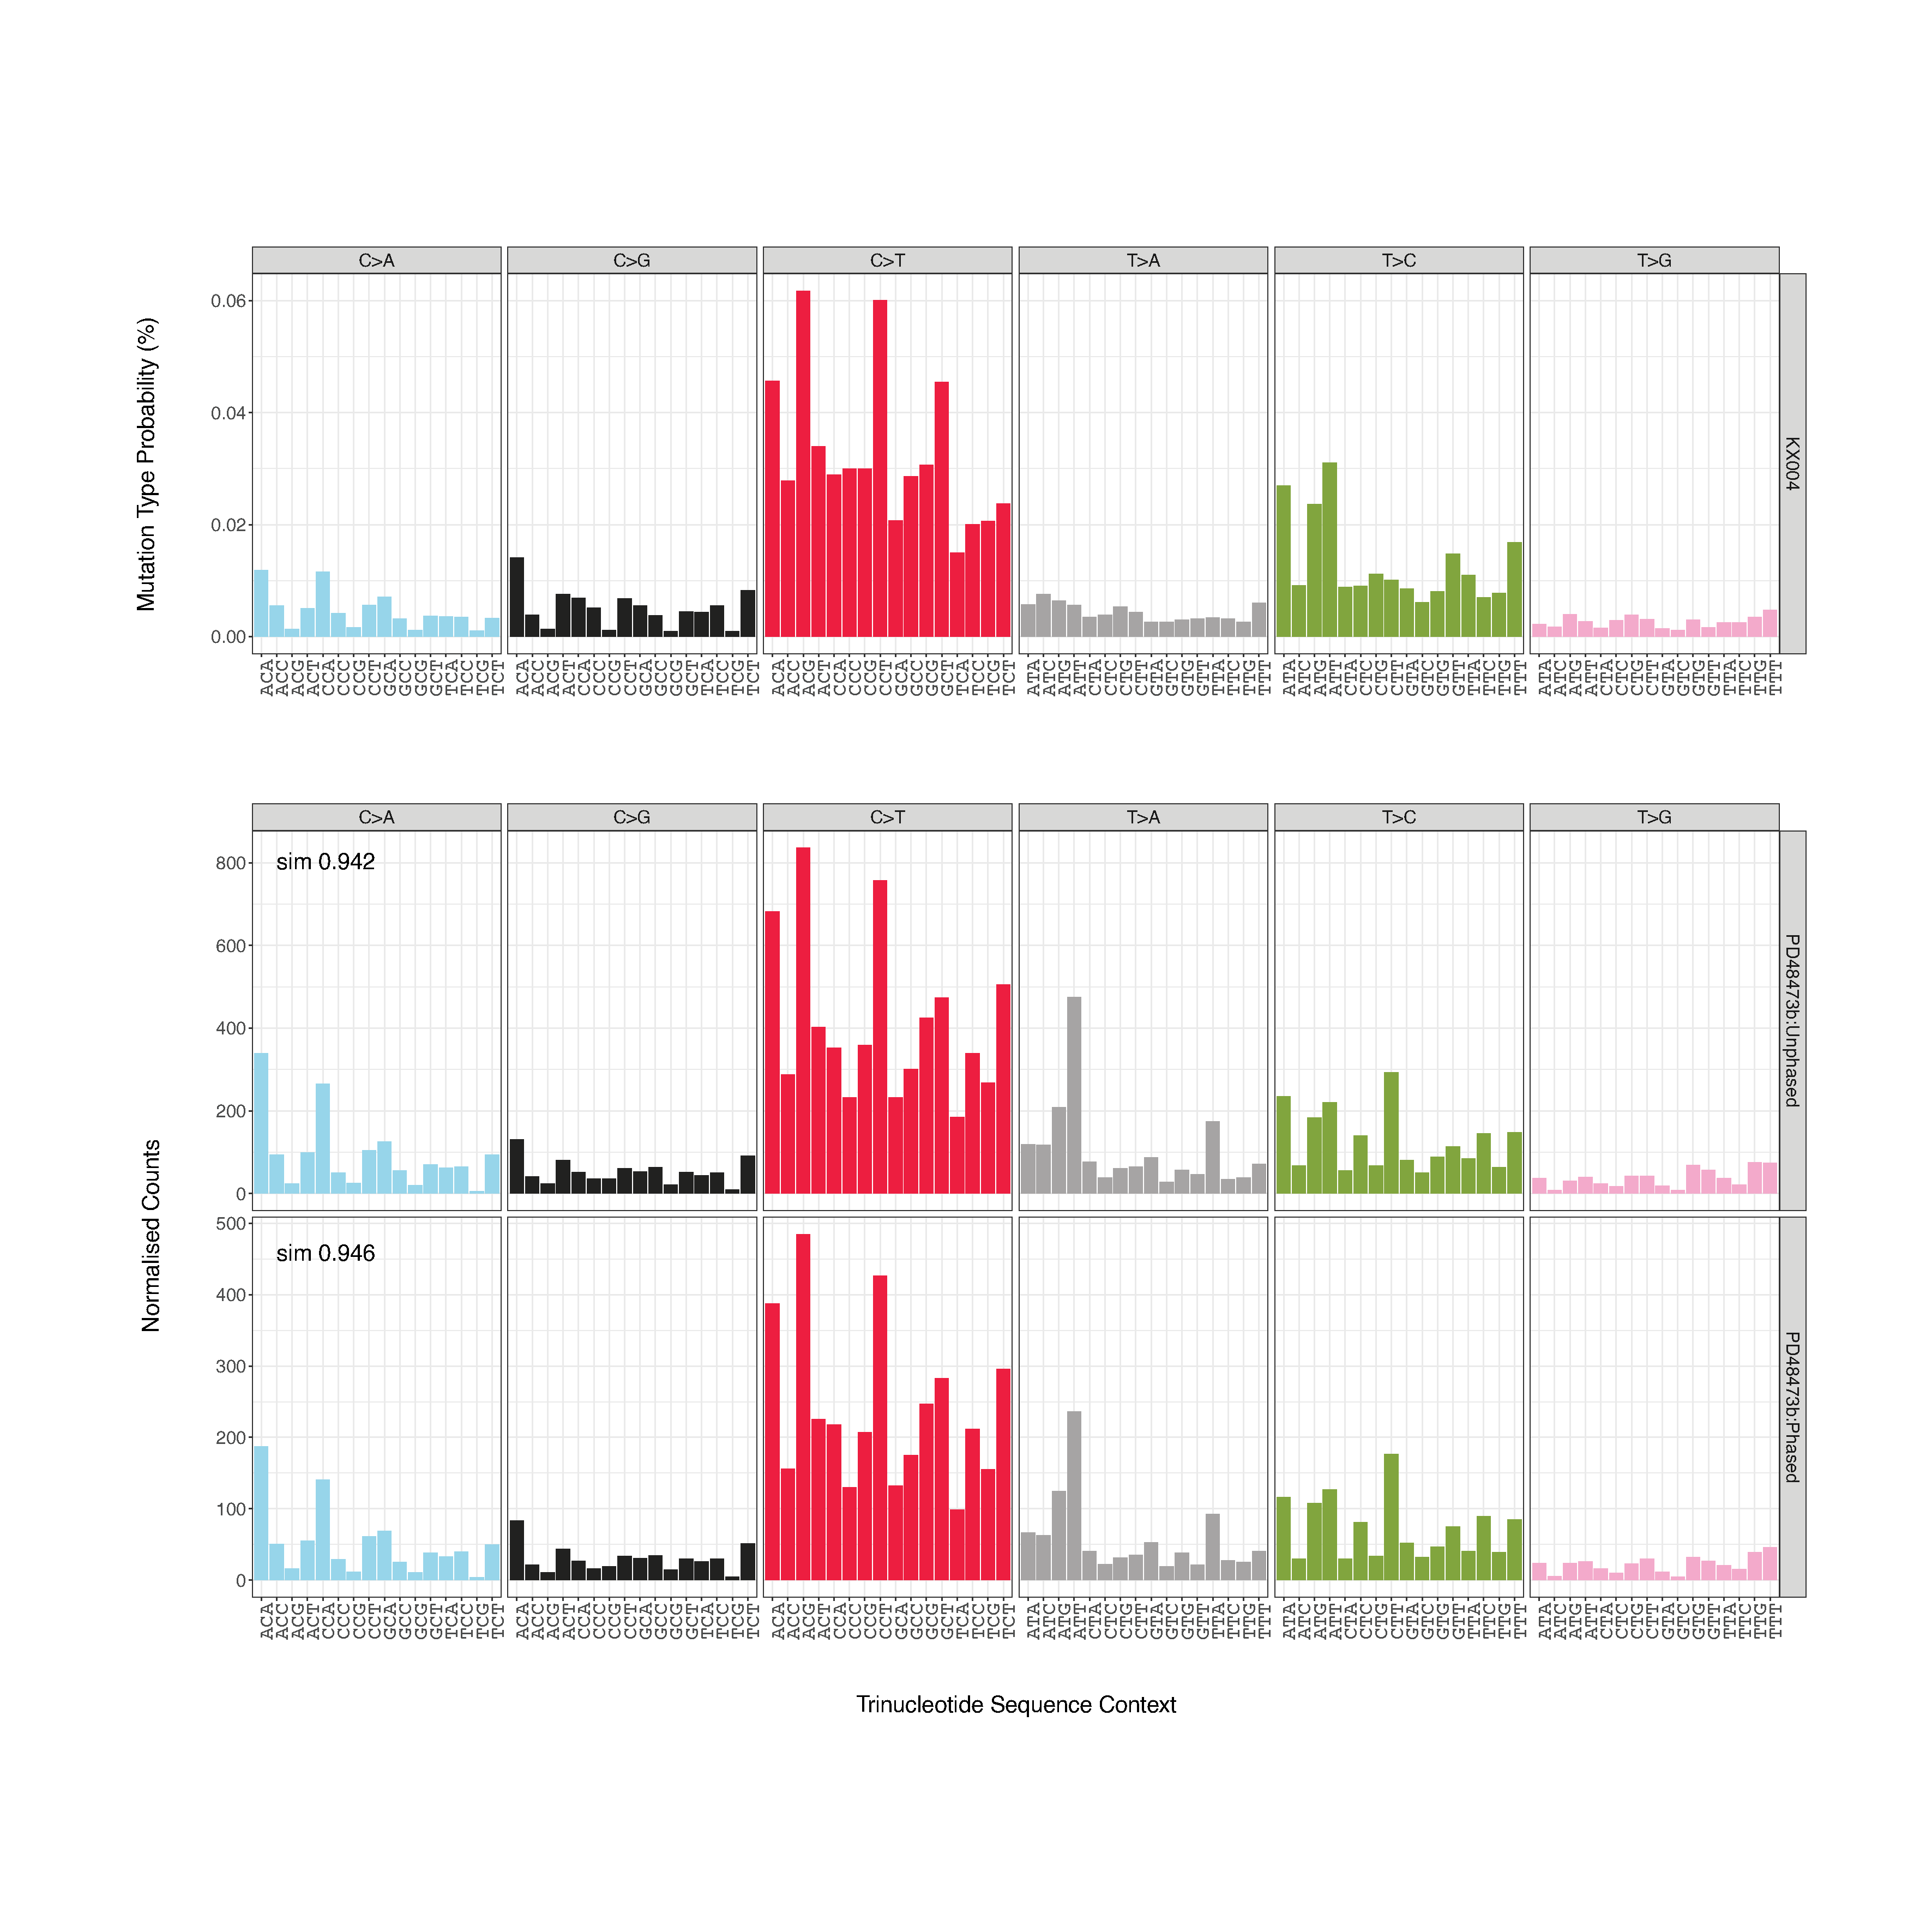
\includegraphics[width=\textwidth]{Vector/hg19.KX001.PD48473b.pdf}
\floatfoot{KX004 mutational spectrum was previously generated from single-cell clone expansion and sequencing \cite{Mitchell2022-ry}}
\end{figure}

In addition, The mutation burden of BC-1, HT-115 and PD48473b samples were calculated to be X, X, X, respectively, consistent with previous estimates \cite{Mitchell2022-ry, Petljak2019-wi}, demonstrating that CCS bases have sufficient base accuracy for rare somatic mutation detection where samples have a high mutation burden or a high somatic mutation rate (Methods) 

Through mutational signature analysis< I was also able to determine the number of true positive mutations and false positive mutations from the called somatic mutations and the number of true negative mutations and false negative mutations from the filtered somatic mutations. These estimates were subsequently used to calculate the sensitivity, specificity, and F1-score for each our sample (Method, Table \ref{}).

\begin{table}[h!]
\caption{}
\label{}
\begin{tabular}{l|>{\centering\arraybackslash}p{2cm}|>{\centering\arraybackslash}p{2cm}|>{\centering\arraybackslash}p{2cm}}
 & BC-1 & HT-115 & PD48473b \\ \hline
Mutation burden per cell & 11,301 & 19,739 & 2,692 \\ \hline
True positive mutations &  &  & \\ \hline 
False positive mutations &  &  & \\ \hline
True negative mutations &  &  & \\ \hline
False negative mutations &  &  & \\ \hline
Sensitivity &  &  & \\ \hline
Specificity &  &  & \\ \hline
F1-score &  &  & \\ \hline
\end{tabular}
\floatfoot{The number of false positive substitutions are included in the mutation burden per cell. Typically, false positive mutations contributes around 700 somatic mutations per cell}
\end{table}

We also selected appropriate hard filter thresholds based on receiver operating characteristic (ROC) curve generated under a range of hard filter conditions (Figure \ref{}) and determined hard filters with the greatest impact on sensitivity based on odds ratio calculated in the absence and presence of the hard filter in question. BQ and GQ score were crucial for somatic mutation detection while other filters had marginally positive impact on somatic mutation sensitivity. We would like to also highlight that somatic mutation detection sensitivity and specificity increased when grch38 was used as a reference genome, reflecting better representation of genetic polymorphisms with improvements in assembly quality (Table). We, unfortunately, could not compare himut with other methods as himut is the first somatic SBS detection method with CCS reads and as somatic mutation detection below 0.1\% VAF has not been technically feasible with standard Illumina reads. 


\subsection{CCS error profile and error rate}

The normal cord blood granulocyte has the lowest mutation burden among our samples, with only 40-50 somatic mutations per cell \cite{Mitchell2022-ry}. CCS bases, unfortunately, does not have sufficient signal-to-noise ratio to enable somatic mutation detection in cord blood sample with high confidence. The number of false positive mutations called from Q93 CCS bases exceeds the number of true positive mutations in the cord blood sample. Hence, mutational spectrum from the cord blood sample is dissimilar to the expected mutational spectrum (Figure \ref{}) and mutational spectrum from the cord blood sample is referred as the CCS error profile. 

%\begin{figure}[h!]
%\caption{}
%\floatfoot{}
%\end{figure}

I was also able to determine the CCS error rate from Q93 CCS base to range from Q60 to Q90 depending on the substitution and the trinucleotide sequence context from the number of false positive mutations (Methods, Figure \ref{}).

%\begin{figure}[h!]
%\caption{}
%\floatfoot{}
%\end{figure}


\subsection{CCS BQ score estimation and recalibration} 

The presence of the CCS error profile across all the samples suggests that these errors originate from a process upstream of somatic mutation detection and hence, library, sequencing and software errors are potential sources of false positive mutations. I was able to pinpoint software errors in BQ score estimation as the main source of false positive mutations using CCS reads with uncapped BQ scores, deepConsensus polished CCS reads and CCS reads with recalibrated BQ scores (Methods). 

CCS BQ score ranges from Q1 to Q93 and the ASCII character encoding format cannot support BQ score above Q93. CCS bases with Q94 base accuracy, for example, will be assigned Q93 BQ score. I, first, assessed whether somatic mutation detection from CCS bases with BQ score greater than Q93 will generate a mutational spectrum that is more consistent with the mutational spectrum that is expected from the normal cord blood granulocyte sample. Unfortunately, the cord blood granulocyte mutational spectrum from higher BQ scores still remained discordant to the expected mutational spectrum (Figure \ref{})

%\begin{figure}
%\caption{}
%\floatfoot{}
%\end{figure}

Google has developed deepConsensus to address some of the issues, but deepConsensus still fails to calculate the correct BQ score and assigns a conservative BQ score to the CCS bases. To generate polished CCS reads, subread are aligned to the CCS read from the same ZMW using actc \cite{}. Afterwards, deepConsensus uses these alignments to polish each CCS read and to assign a BQ score between Q1 and Q50. As discussed above, I estimated that Q93 CCS base accuracy ranges from Q60 to Q90 depending on the substitution and trinucleotide sequence context. I, hence, think that CCS BQ score estimates from deepConsensus are also inaccurate. In addition, somatic mutation detection with Q50 CCS bases from deepConsensus polished CCS reads also does not yield the expected mutational spectrum, corroborating the above observation (Figure \ref{}). I conjecture that their model does not consider somatic mutations and in fact, classifies somatic mutations as errors, which leads to inaccurate BQ score estimations.  

%\begin{figure}
%\caption{}
%\floatfoot{}
%\end{figure}

Under the assumption SMRT sequencing errors are random and that inaccurate BQ score estimation is the main source of false positive mutations. To test this hypothesis, CCS bases with unanimous support from subreads were identified and were used for somatic mutation detection (Methods). The expected mutational spectrum was recovered from the cord blood granulocyte sample, suggesting that in accurate BQ score estimation and not sequencing error is the primary source of false positive mutations (Figure \ref{}). 

%\begin{figure}
%\caption{}
%\floatfoot{}
%\end{figure}


\section{Conclusion}

Here, I determined that Q93 CCS bases have base accuracy that ranges from Q60 to Q90 depending on the substitution and the trinucleotide sequence context. Hence, a subset of CCS bases has sufficient base accuracy to enable single molecule somatic mutation detection. I use samples with single ongoing somatic mutational processes to demonstrate that single molecule somatic mutation detection is indeed possible with CCS reads and that mutational spectrum produced from the aggregate of somatic mutations is concordant with the expected mutational signature from each positive control sample. In addition, I also show that inaccurate BQ score estimation to be the primary source of false positive mutations and that BQ score can be recalibrated to address this issue. 

\section{Materials and Methods}

\subsection{CCS library preparation and sequencing}


BC-1 and HT-115 cell lines were cultured at 37 \textcelsius, 5\% CO2 in RPMI and DMEM media, respectively, supplemented with 5\% fetal bovine serum and penicillin. Umbilical blood from a newborn female (PD47269d) and peripheral blood sample of an 82-year-old female (PD48473b) were collected in 40-60mL lithium-heparin tubes and blood granulocytes were subsequently isolated using Lymphophorep. High molecular weight (HMW) DNA from BC-1 and HT-115 cell line and PD47269d and PD484873b blood granulocytes were extracted using Qiagen MagAttract HMW DNA extraction kit (67563) and sheared to 16-20kb DNA fragments using Megaruptor 3 system (B06010003) with speed setting 30. CCS sequencing libraries were constructed according to the CCS library preparation protocol 1.0 (100-222-300), and the libraries were sequenced using a Sequel IIe instrument at the Wellcome Sanger Institute. 

\subsection{CCS read alignment and germline mutation detection}
CCS reads with adapter sequences were identified with HiFiAdapterFilt \cite{Sim2022-pi} and were removed from downstream sequence analysis. CCS reads were aligned to the human reference genome (b37 and grch38) with minimap2 (version 2.24-r1155-dirty) with default parameters for CCS read alignment (-ax map-hifi --cs=short) \cite{Li2018-am} and primary alignments were selected, compressed, merged, and sorted with samtools (version 1.6) \cite{Li2009-qp}. Germline SNPs and indels were detected with deepvariant (version 1.1.0) \cite{Poplin2018-ub}. VCF files were compressed and indexed with tabix \cite{Li2011-zj} and left aligned and normalised with bcftools (version 1.17-7-g097bda6) \cite{Li2011-ag}


\subsection{CCS empirical base quality score calculation}

To assess the potential for somatic mutation detection with CCS reads, the accuracy of the BQ score estimate was assessed using CCS reads from cord blood granulocytes. The number of matches and mismatches were counted for each BQ score to calculate the empirical BQ score. Reference allele and germline SNPs were considered as matches, while all other SBS were classified as mismatches. Germline mutation detection using himut is described below. Germline SNPs with genotype quality (GQ) score below 20 and read depth above maximum depth threshold $4d + \sqrt{d}$, where $d$ is the average read depth, were excluded from analysis. Phred-scaled quality scores were calculated based on the number of matches and mismatches for each BQ score (eq \ref{eq:empirical-bq}).

\begin{equation} \label{eq:empirical-bq}
\text{empirical BQ} = -10 \times \log_{10} \Big( \frac{\text{mismatch count}}{\text{match count}} \Big)
\end{equation}

\subsection{Germline and somatic mutation detection}

To detect germline and somatic mutations from bulk normal tissue, himut leverages CCS read length and base accuracy for somatic mutation candidate detection and applies a set of hard filters to distinguish potential errors from somatic mutations. Himut uses pysam \cite{pysam}, pyfastx \cite{Du2021-ya} and cyvcf2 \cite{Pedersen2017-ld} to process BAM, FASTA/Q and VCF files, respectively. Himut also uses the multiprocessing Python package \cite{multiprocessing} to enable parallel processing of all the chromosomes. 

Upon initiation, read alignments are first randomly sampled from each target chromosome to compute the lower and upper bound read length and maximum read depth threshold $4d + \sqrt{d}$ where $d$ is the average read depth \cite{Li2014-ra}. Afterwards, CCS reads with average read accuracy, mapping quality score (MAPQ) and sequence identity equal or greater than the predefined thresholds are selected and SBS candidates are collected from these reads. Average read accuracy is the mean BQ score of the CCS read (eq \ref{eq:average-read-accuracy}).

\begin{equation} \label{eq:average-read-accuracy}
\text{Average read accuracy} = \frac{\sum^{l}_{i}b_{i}}{l} \smallskip
\end{equation}

where $b$ is the BQ score for the CCS base index $i$ and $l$ is the CCS read length.

Sequence identity is the ratio of matching bases relative to the total number of aligned bases (eq \ref{eq:sequence-identity}).  

\begin{equation} \label{eq:sequence-identity}
\text{Sequence identity} = \frac{\text{match}}{\text{alignment length}} \smallskip
\end{equation}

In addition, CCS read length must be between the lower and upper bound read length to prevent somatic mutation detection from erroneously fragmented or concatenated reads. The lower and upper bound read length is defined as such (eq \ref{eq:lower-upper-read-length}): 

\begin{equation}
\begin{aligned} 
\text{Lower bound read length} &= \mu - 2\sigma \\
\text{Upper bound read length} &= \mu + 2\sigma 
\end{aligned}
\label{eq:lower-upper-read-length}
\end{equation}

where $\mu$ is the average CCS read length and $\sigma$ is the standard deviation for the read length. 

The default read-level thresholds for himut are defined below:

\begin{enumerate}
\item The average read accuracy needs to be equal or greater than the minimum average read accuracy (default: -{}-min\_qv = 30)
\item MAPQ score of the read needs to be greater than the minimum MAPQ score (default: -{}-min\_mapq = 60)
\item Sequence identity of the read needs to be equal or greater than the minimum sequence identity threshold (default: -{}-min\_sequence\_identity 0.99)
\item CCS read length needs to be between the lower ($\mu - 2\sigma$) and upper bound ($\mu + 2\sigma$) read length.
\end{enumerate}

Subsequently, a naive Bayesian genotyper is used to determine whether the data $(D)$ only supports the variant as a germline mutation or whether the data support both a germline variant and a somatic mutation candidate simultaneously (eq \ref{eq:bayes-rule}):

\begin{equation} \label{eq:bayes-rule}
P(G|D) = \frac{P(G)P(D|G)}{P(D)} \smallskip
\end{equation}

where there are 10 possible genotypes $G \in (\text{AA, CA, CC, CT, GA, GC, GG, GT, TA, TT})$. $P(G)$ is the prior probability of observing the genotype and is dependent on whether the genotype is heterozygous, heterozygous alternative (tri-allelic), homozygous alternative or homozygous reference allele with respect to the reference base (eq \ref{eq:genotype-prior}).  

\begin{equation} \label{eq:genotype-prior}
 P(G)= 
 	\begin{dcases}
    	\theta & \text{if } G = g_{\text{het}} \\
	    \frac{\theta}{2} & \text{if } G = g_{\text{hetalt}} \\
		\theta^{2} & \text{if } G = g_{\text{homalt}} \\
		1 - \frac{3\theta}{2} - \theta^{2} & \text{if } G = g_{\text{homref}} \\
	\end{dcases} \smallskip
\end{equation}

where $\theta$ is the expected germline SNP frequency and the default $\theta$ is set as $1\times10^{-3}$, the expected human germline SNP frequency \cite{1000_Genomes_Project_Consortium2012-rj}. 

$D$ is the data that represents the pileup of read bases and corresponding sequencing error probabilities for each base at the substitution site. $P(D)$ is a constant across all the possible genotypes and is ignored. $P(D|G)$ is the probability of observing the data given the genotype. 

Binomial likelihood is calculated for each genotype under the assumption that sequencing errors and read sampling is independent and identically distributed (eq \ref{eq:binomial-likelihood}):

\begin{equation} \label{eq:binomial-likelihood}
P(D|G) =  
	\begin{dcases}
    	\frac{1}{2^n}\prod_{i}^{n} (P(b_{i}|G_1) + P(b_{i}|G_2) & \text{if } G = g_{\text{het}} \text{ or } g_{\text{hetalt}} \\
	    \prod_{i}^{n} P(b_{i}|G) & \text{if } G = g_{\text{homalt}} \text{ or } g_{\text{homref}} \\
	\end{dcases}
\end{equation}

where $P(b|G)$ is the probability of observing the base given the genotype (eq \ref{eq:base-error-rate})

\begin{equation} \label{eq:base-error-rate}
P(b_{i}|G) = P(b_{i}|A) = 
	\begin{dcases}
    	1 - \epsilon_{i} & \text{if } b_{i} \in A \\
	    \frac{\epsilon_{i}}{3} & \text{if } b_{i} \not\in A \\
	\end{dcases} \smallskip
\end{equation}

where $b$ is the CCS base covering the target locus, $\epsilon$ is the corresponding sequencing error probability and $A$ is the allele of the genotype. In practice, all calculations are performed in log scale. Phred scaled likelihood (PL) is calculated for all the possible genotypes (eq \ref{eq:phred-scaled-posterior-probability}):

\begin{equation} \label{eq:phred-scaled-posterior-probability}
\text{PL} = -10\log_{10}P(G|D) 
\end{equation}

and PL for each genotype is normalised using the lowest PL (eq \ref{eq:normalised-PL}).

\begin{equation} \label{eq:normalised-PL}
\text{normalised PL} = [\text{PL}_{i}, \text{PL}_{i+1}, \ldots, \text{PL}_{10}] - \text{PL}_{i}
\end{equation}

where PL is assumed to be sorted from the smallest to the largest. The genotype with the lowest PL is selected as the germline genotype. Genotype quality (GQ) score of the selected germline genotype is the difference between the second lowest normalised PL and the lowest normalised PL. If the data only provides evidence for a germline mutation, the next SBS is then considered for somatic mutation detection. If the data support the presence of both a germline mutation and a somatic mutation candidate, a set of hard filters are applied to call somatic mutations. 

A VCF file with common SNPs (>1\% major allele frequencies) and a Panel of Normal (PoN) VCF file can also be optionally provided to exclude somatic mutation candidates arising from DNA contamination and systematic bioinformatics error, respectively. In addition, a VCF file with haplotype-phased hetSNPs can be provided to limit somatic mutation detection from haplotype phased regions. 

The default base-level conditions for himut are defined below: 

\begin{enumerate}
\item If the germline mutation is a heterozygous, heterozygous alternative or homozygous alternative allele, somatic mutation candidate is excluded from the downstream analysis as somatic reversions are not considered. Somatic mutation detection, hence, is restricted to a locus with a homozygous reference allele to prevent the misclassification of heterozygous mutation as a somatic mutation.
\item The GQ score for the homozygous reference allele needs to be above the minimum GQ score threshold (default: -{}-min\_gq = 20).
\item The BQ score of the somatic mutation candidate needs to be above the minimum BQ score threshold (default: -{}-min\_bq = 93).
\item Indels must be absent from the SBS locus.
\item The read depth of the target locus needs to be below the maximum depth threshold, which is dependent on the sample sequence coverage. 
\item The reference allele count and the alternative allele count need to be above the minimum reference allele count (default: -{}-min\_ref\_count = 3) and minimum alternative allele count (default: -{}-min\_alt\_count = 1). This condition is not required if the sample has sufficient sequence coverage as the GQ score is positively correlated with sequence coverage.
\item CCS reads with adapter sequences might still be present in the BAM file and misalignment of residual adapter sequences can generate somatic mutation candidates. Hence, candidates located near the start and end of reads are filtered  (default: -{}-min\_trim = 0.01).
\item The number of mismatches adjacent to the candidate needs to be below the maximum mismatch count (default: -{}-max\_mismatch\_count = 0) within a given mismatch window (default: -{}-mismatch\_window\_size = 20) as an alignment error can be misclassified as a somatic mutation. The –{}-mismatch\_window\_size parameter is used to extend the mismatch window upstream and downstream of the SBS call position. If the extension is beyond the 5’ or 3’ end of the read, the number of bases extended beyond the 5’ end of the read, for example, is used to extend the 3’ end of the mismatch window.
\item If a VCF file with haplotype phased hetSNPs are provided for somatic mutation detection, CCS read with the somatic mutation candidate has to be identical to one of the two consensus haplotype blocks. In addition, the number of CCS reads, without the somatic mutations, from both haplotypes must be greater than the minimum number of haplotype count (default: --min\_hap\_count = 3). Furthermore, if more than one read has the somatic mutation candidate, CCS reads with the somatic mutation candidate must share the same haplotype. Haplotype phased somatic mutation detection prevents the misclassification of hetSNPs as somatic mutations. 
\item Somatic mutation candidates found in either the PoN VCF file or VCF file with common SNPs is excluded from downstream sequence analysis. 
\end{enumerate}

Somatic mutations were called in both positive and negative control samples using himut with default parameters. Somatic mutation detection was also restricted to the autosomes as sex chromosomes are enriched for misassembled regions and repetitive sequences \cite{Skaletsky2003-sr}.


\subsection{Panel of Normal construction}

To generate a PoN VCF file, publicly available CCS dataset from 11 normal unrelated individuals was collected \cite{Zook2019-pm} (Table \ref{tab:pon-fastq-statistics}) and processed as described above to generate merged and sorted primary read alignments. Afterwards, somatic mutations were identified from these samples using himut with less stringent parameters (--min\_qv 20 -{}-min\_mapq 30 –{}-min\_trim 0 –{}-min\_sequence\_identity = 0.8 -{}-min\_gq –{}-min\_bq = 20) to maximise the number of mutations called from each sample. 

\begin{table}[h!]
\caption{PoN sample FASTQ statistics}
\label{tab:pon-fastq-statistics}
\begin{adjustbox}{max width=1.1\textwidth,center}
\begin{tabular}{c|c|c|c|c}
& Number of CCS reads & Average CCS read length(bp) & BQ93 proportion (\%) & Sequence coverage \\ \hline
HG001 & 9,076,967 & 9,963 & 58.9 & 30.1 \\ \hline
HG003 & 12,490,825 & 15,423 & 60.6 & 64.2 \\ \hline
HG004 & 11,528,550 & 16,044 & 57.0 & 61.6 \\ \hline
HG005 & 9,425,306 & 10,423 & 58.1 & 32.7  \\ \hline
HG00514 & 4,500,935 & 16,988 & 45.1 & 25.5 \\ \hline
HG00731 & 9,286,164 & 11,133 & 58.0 & 34.5 \\ \hline
HG00732 & 9,566,270 & 14,935 & 45.2 & 47.6 \\ \hline
HG00733 & 7,657,979 & 13,552 & 51.8 & 34.6 \\ \hline
NA19238 & 1,320,856 & 11,420 & 53.8 & 5.0 \\ \hline
NA19239 & 2,661,222 & 15,358 & 44.7 & 13.6 \\ \hline
NA19240 & 5,695,556 & 12,743 & 52.3 & 24.1 \\ \hline
\end{tabular}
\end{adjustbox}
\end{table}

The number of samples in the PoN VCF is currently limited to the number of publicly available CCS dataset. As the number of CCS sequenced samples increases, the power to distinguish errors from somatic mutations will also increase in the future.  

\subsection{Germline mutation haplotype phasing}

A haplotype is defined as a group of genetic variants that are inherited together from a single parent. Haplotype phasing is treated as a graph algorithm problem where each hetSNP is a node in a graph and there is an edge between a pair of haplotype consistent hetSNPs. A single CCS read spans multiple heterozygous SNPs and evidence from multiple CCS reads can determine whether a pair of hetSNPs is haplotype consistent (p < 0.0001, one-sided binomial test) . If a pair of hetSNP is haplotype consistent, a pair of hetSNP exists in cis-configuration or trans-configuration (Figure \ref{figure:cis-trans-configuration}). A haplotype inconsistent pair of hetSNP results from non-biological sources. Haplotype consistency is measured between all possible hetSNP pairs and hetSNPs that are haplotype consistent with at least 20\% of their possible pairs are connected through breadth-first search algorithm to construct haplotype blocks. Himut accepts as input a VCF file with germline mutations and returns a VCF file with haplotype phased hetSNPs.

\begin{figure}[htbp!]
\caption{cis- and trans-configuration for a hetSNP pair}
\label{figure:cis-trans-configuration}
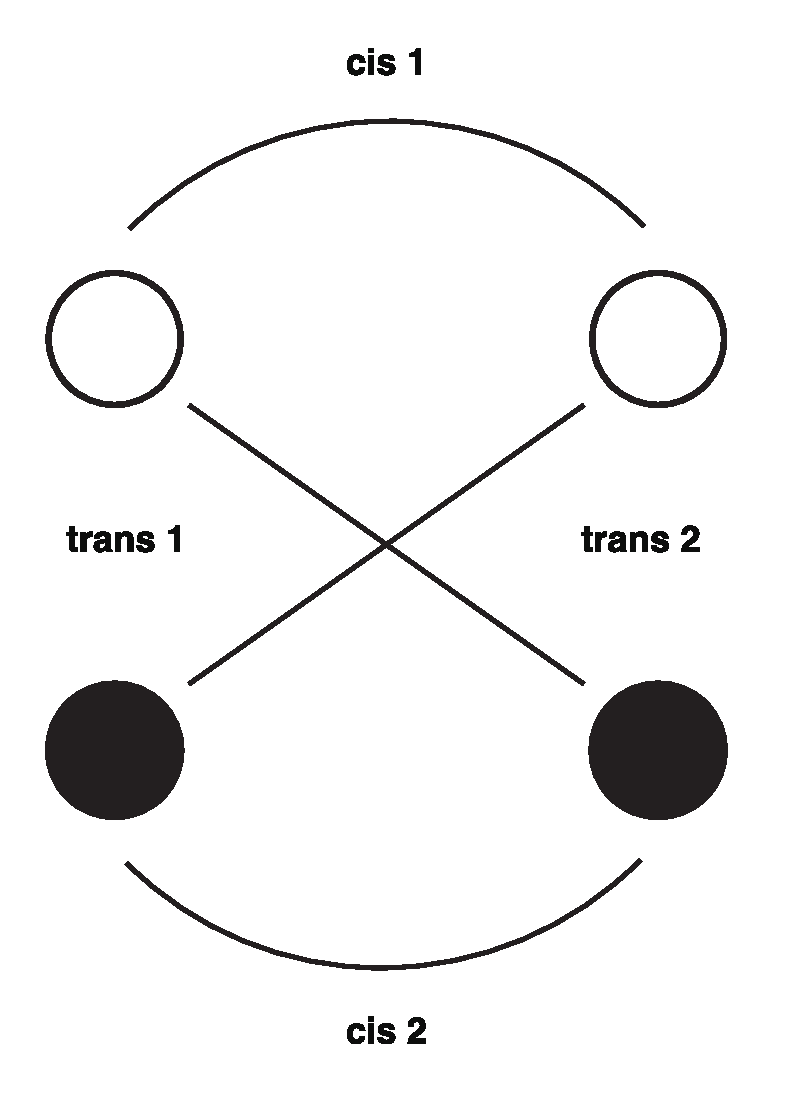
\includegraphics[width=0.4\textwidth]{Vector/cis_trans_configuration.pdf}
\end{figure}

\subsection{Haplotype phased somatic mutation detection}

CCS reads are assigned to a haplotype block to enable haplotype phased somatic mutation detection. To be allocated to a haplotype block, a CCS read must be within a haplotype block (and not between two haplotype blocks) and have haplotype identical to the consensus haplotype as defined in the haplotype block. Therefore, somatic mutations are not phased through adjacent hetSNPs and instead phased CCS reads are used for somatic mutation detection. 

\subsection{Somatic mutation count normalisation}
To normalise the number of substitutions per trinucleotide sequence context, the SBS96 classification system and the same conditions as somatic mutation detection are used to calculate the number of callable reference and CCS bases. I would like to highlight that only the reference bases where homozygous reference allele has been called without an indel is considered as a callable reference base. 

Under the SBS96 classification, SBS is categorised according to 6 possible substitution types in the pyrimidine context (C>A, C>G, C>T, T>A, T>C and T>G) and 16 possible trinucleotide sequence context derived from the 4 possible bases upstream and downstream of the substitution. 

The frequency of each trinucleotide is calculated for the reference $f^{g}_{i}$, callable reference $f^{g_{\text{callable}}}_{i}$, and callable CCS $f^{\text{CCS}}_{i}$ bases from the reference genome FASTA file, the number of callable reference bases and the number of callable CCS bases, respectively (eq \ref{eq:trinucleotide-frequency}). 

\begin{equation} \label{eq:trinucleotide-frequency}
f_{i} = \frac{t_{i}}{\sum^{32}_{i=1} t_{i}}
\end{equation}

where $t$ denotes a specific trinucleotide. There are 32 possible trinucleotide sequence contexts where pyrimidine is the middle base. 

Afterwards, the number of somatic mutations is normalised with the ratio of reference to callable reference trinucleotide frequency and the ratio of callable reference and callable CCS base trinucleotide frequency according to the substitution and the trinucleotide sequence context. ACA>A somatic mutation count, for example, is normalised as follows (eq \ref{eq:sbs96-normalisation}):

\begin{equation} \label{eq:sbs96-normalisation}
S'_{\text{ACA>AAA}} = S_{\text{ACA>AAA}} \times r^{g}_{\text{ACA}} \times r^{\text{callable}}_{\text{ACA}} 
\end{equation}

where $S'_{\text{ACA>AAA}}$ is the normalised substitution count, $S_{\text{ACA>AAA}}$ is the raw substitution count, $r^{g}_{\text{ACA}}$ is the ratio of reference to callable reference ACA frequency and $r^{\text{callable}}_{\text{ACA}}$ is the ratio of callable reference and CCS base ACA frequency. 

The ratio of reference to callable reference trinucleotide frequency and the ratio of callable reference and CCS base trinucleotide frequency are calculated as follows (eq \ref{eq:trinucleotide-ratio}):

\begin{equation}
\begin{aligned} 
r^{g}_{i} &= \frac{f^{g_{\text{callable}}}_{i}}{f^{g}_{i}} \\[1em]
r^{\text{callable}}_{i} &= \frac{f^{g_{\text{callable}}}_{i}}{f^{\text{CCS}_{\text{callable}}}_{i}}
\end{aligned}
\label{eq:trinucleotide-ratio}
\end{equation}

\subsection{Mutation burden calculation}

The somatic mutation rate is calculated for each trinucleotide sequence context from the normalised somatic mutation counts and the number of callable CCS bases (eq \ref{eq:trinucleotide-somatic-mutation-rate})

\begin{equation} \label{eq:trinucleotide-somatic-mutation-rate}
m_{\text{ACA}} = \frac{S'_{\text{ACA>AAA}} + S'_{\text{ACA>AGA}} + S'_{\text{ACA>ATA}}}{t^{\text{CCS}_{\text{callable}}}_{\text{ACA}}} 
\end{equation}

where $m_{\text{ACA}}$ is the somatic mutation rate for the ACA trinucleotide sequence context. 

To calculate the mutation burden per cell, mutation burden per genome is calculated from the trinucleotide sequence context specific somatic mutation rate and the number of trinucleotides in the reference FASTA file. Afterwards, mutation burden per genome is adjusted with the ploidy of the sample to derive the mutation burden per cell (eq \ref{eq:mutation-burden-per-cell})

\begin{equation} \label{eq:mutation-burden-per-cell}
g_{\text{burden}} = n * (\sum^{32}_{i=1} m_{i} * t^{g}_{i})
\end{equation}

where $n$ is the ploidy of the sample, $m_{i}$ is the trinucleotide sequence context somatic mutation rate and $t^{g}_{i}$ is the number of trinucleotides in the reference genome.

\subsection{Concordance between mutational spectrum and expected mutational signature}

In order to determine the degree of concordance between the mutational spectrum derived from the sample and the expected mutational signature from the sample, cosine similarity is measured (equation \ref{eq:cosine-similarity})

\begin{equation} 
\label{eq:cosine-similarity}
\text{Cosine similarity} (A,B) = \frac{\sum^{n}_{i=1}A_{i}B_{i}}{\sqrt{\sum^{n}_{i=1}A^{2}_{i}}\sqrt{\sum^{n}_{i=1}B^{2}_{i}}}
\end{equation}

where $A$ and $B$ are two mutational spectra to be compared. Both $A$ and $B$ are vectors with non-negative integers and have the same number of mutation types. Cosine similarity ranges from 0 to 1. A cosine similarity of 0 means that the two mutational spectra are independent while a cosine similarity of 1 indicates that the two mutational spectra are identical. 

BC-1 mutational spectrum was compared with SBS2 mutational signature, HT-115 mutational spectrum was compared with linear combination of SBS10a, SBS10b and SBS28 mutational signatures and PD48473b mutational spectrum was compared with KX004 mutational spectrum.

\subsection{Somatic mutation detection sensitivity and specificity}

The number of true positive (TP), false positive (FP), true negative (TN) and false negative (FN) somatic mutations were calculated from filtered and passed somatic mutations using MutationalPatterns R package \cite{Blokzijl2018-jo}. Afterwards, sensitivity, specificity and F1-score were derived as such: (equation \ref{eq:sensitivity-specificity})

\begin{equation}
\begin{aligned} 
\text{Sensitivity} &= \frac{\text{TP}}{\text{TP+FN}} \\[1em] 
\bigskip \text{Specificity} &= \frac{\text{TN}}{\text{TN+FP}} \\[1em] 
\text{F1-score} &= \frac{\text{2TP}}{\text{2TP+FP+FN}}
\end{aligned}
\label{eq:sensitivity-specificity}
\end{equation}



\subsection{CCS error rate per trinucleotide sequence context}

To calculate the substitution error rate per trinucleotide sequence context, raw subreads BAM file from the normal cord blood granulocyte was processed to return a new subreads BAM file with 10 full-length subreads per ZMW. A full-length subread is defined as a subread that has a length between 0.8 $\times$ median subread length and 1.2 $\times$ median subread length. The first and the last subread are excluded from the new BAM file. 

CCS reads were re-generated from the new subreads BAM file using pbccs (v 6.3.0) \cite{}. Because the number of subreads per CCS read influences the CCS BQ score estimate and because the increase in the number of CCS reads have negative returns to CCS BQ score estimate, the number of subreads were set as a constant (discussed and demonstrated further in chapter 3). The re-generated CCS reads were processed as described above for somatic mutation detection and SBS96 count normalisation. 

Somatic mutations detected from the cord blood granulocyte are attributable to either the clock-like mutational process or errors. As the number of called somatic mutations greatly exceeds the expected number of somatic mutations from the sample (40 – 50 somatic mutations per cell) \cite{Osorio2018-mh, Mitchell2022-ry}, the, false positive mutations are assumed to be enriched in the somatic mutation catalogue. 
 
To accurately ascertain the number of false positive mutations, the number of true positive somatic mutations were first estimated for each SBS96 classification from the number of callable trinucleotide bases and the cord blood somatic mutational process (eq \ref{eq:mutation-count-estimation}). 

\begin{equation} \label{eq:mutation-count-estimation}
\text{cord blood } S_{\text{ACA>AAA}}= p_{\text{ACA>AAA}} * t^{\text{CCS}}_{\text{ACA}})
\end{equation}

where $S_{\text{ACA>AAA}}$ is the estimate of the number of C>A substitution in the ACA trinucleotide sequence context. $p_{\text{ACA>AAA}}$ is the probability that C>A substitution will occur in the ACA trinucleotide sequence context and is derived from previous single-cell clone expansion and sequencing study \cite{Mitchell2022-ry}. $t^{\text{CCS}}_{\text{ACA}}$ is the number of ACA trinucleotides from which somatic mutations could have been called from.

The normalised SBS96 counts were adjusted with the expected number of somatic mutations from each trinucleotide sequence context and the resulting estimate of the number of false positive mutations was divided by the number of callable CCS bases to obtain the substitution error rate per trinucleotide sequence context (eq \ref{eq:substitution-error-rate-per-trinucleotide-sequence-context}). 

\begin{equation} \label{eq:substitution-error-rate-per-trinucleotide-sequence-context}
\text{C>A error rate for ACA context} = \frac{\text{false positive } S_{\text{ACA>AAA}}}{t^{\text{CCS}}_{\text{ACA}}}
\end{equation}





\subsection{CCS base quality score recalibration}

To re-calculate the CCS BQ scores, actc \cite{actc} was used to align subreads to CCS reads from the same ZMW and the resulting BAM file was provided as input towards deepConsensus (v1.1.0, 37fb6b2) \cite{Baid2022-or} and for partial order alignment based BQ score recalibration. Afterwards, CCS reads with recalibrated BQ scores were processed as described above to call somatic mutations and assess. 

\subsubsection{DeepConsensus}

DeepConsensus accepts as input the actc BAM file where subreads have been aligned to CCS read from the same ZMW and BAM file with CCS reads and returns as output polished CCS reads with recalibrated BQ score. 

\subsubsection{CCS bases with unanimous support from subread bases}

To find CCS bases where all the subread bases support the CCS base, actc BAM file is processed to determine the median subread length per ZMW, to determine the sequence orientation of subreads relative to the CCS read and return a FASTA file per ZMW with CCS reads and 10 full-length subreads. As before, a full-length subread is defined as a subread that has a length between 0.8 $\times$ median subread length and $1.2 \times$ median subread length, and first and last subreads are not returned to the FASTA file. A partial order alignment is constructed from each FASTA file using abPOA \cite{Gao2021-nf}. The resulting multiple sequence alignment is analysed to identify CCS bases where all the subread bases support the CCS base and Q93 BQ score is assigned to the CCS base, while a BQ score is calculated as such for all other CCS base (equation \ref{eq:bq-score-calculation})

\begin{equation}
\text{BQ} = -10\log10 \Biggl(\epsilon^k {n \choose k}\Biggl)
\label{eq:bq-score-calculation}
\end{equation}

where $\epsilon$ is a constant error prior of 0.1 for all bases, $n$ is the number of subreads, which is also a constant at 10, and $k$ is the number of subreads supporting the CCS base.

